\chapter{Results of the averaging learning on 3 ideal datasets}
\label{app:C}
The figures shown in this appendix serve as a completion on the figures that were presented in the discussion of section \ref{s:averaging_method}. It concerns the results of the learning algorithm that learns from three ideal datasets with the amount of control points $N$ equal to 1000 and time limit set to $30 \hspace{1mm}s$.\\ First the resulting kinematic signals of the bicycle model during the different lane changes are shown. It should be noted that Figure \ref{fig:app_delta} and \ref{fig:app_delta_dot} show the angle of the front wheel of the bicycle model. In order to obtain the steerwheelangle, this relation is linearised by the factor $Gs = 16.96$ which means that $\delta_{SWA} = Gs\cdot\delta_{front}$. Further Figure \ref{fig:app_conv} displays the convergence during the learning process and plots $\bm{f}_{rel}$ over the iterations. Figure \ref{fig:app_grad} shows the absolute difference between the learned and observed features. In Figure\ref{fig:app_weights} the learning of the weights towards the final ones are presented. Figure \ref{fig:app_update} gives the difference of current weight with respect to the previous one and as last Figure \ref{fig:app_multigrad} shows which of the three RPROP cases that is used in order to update a certain weight. 

 
\begin{figure}[h!]
	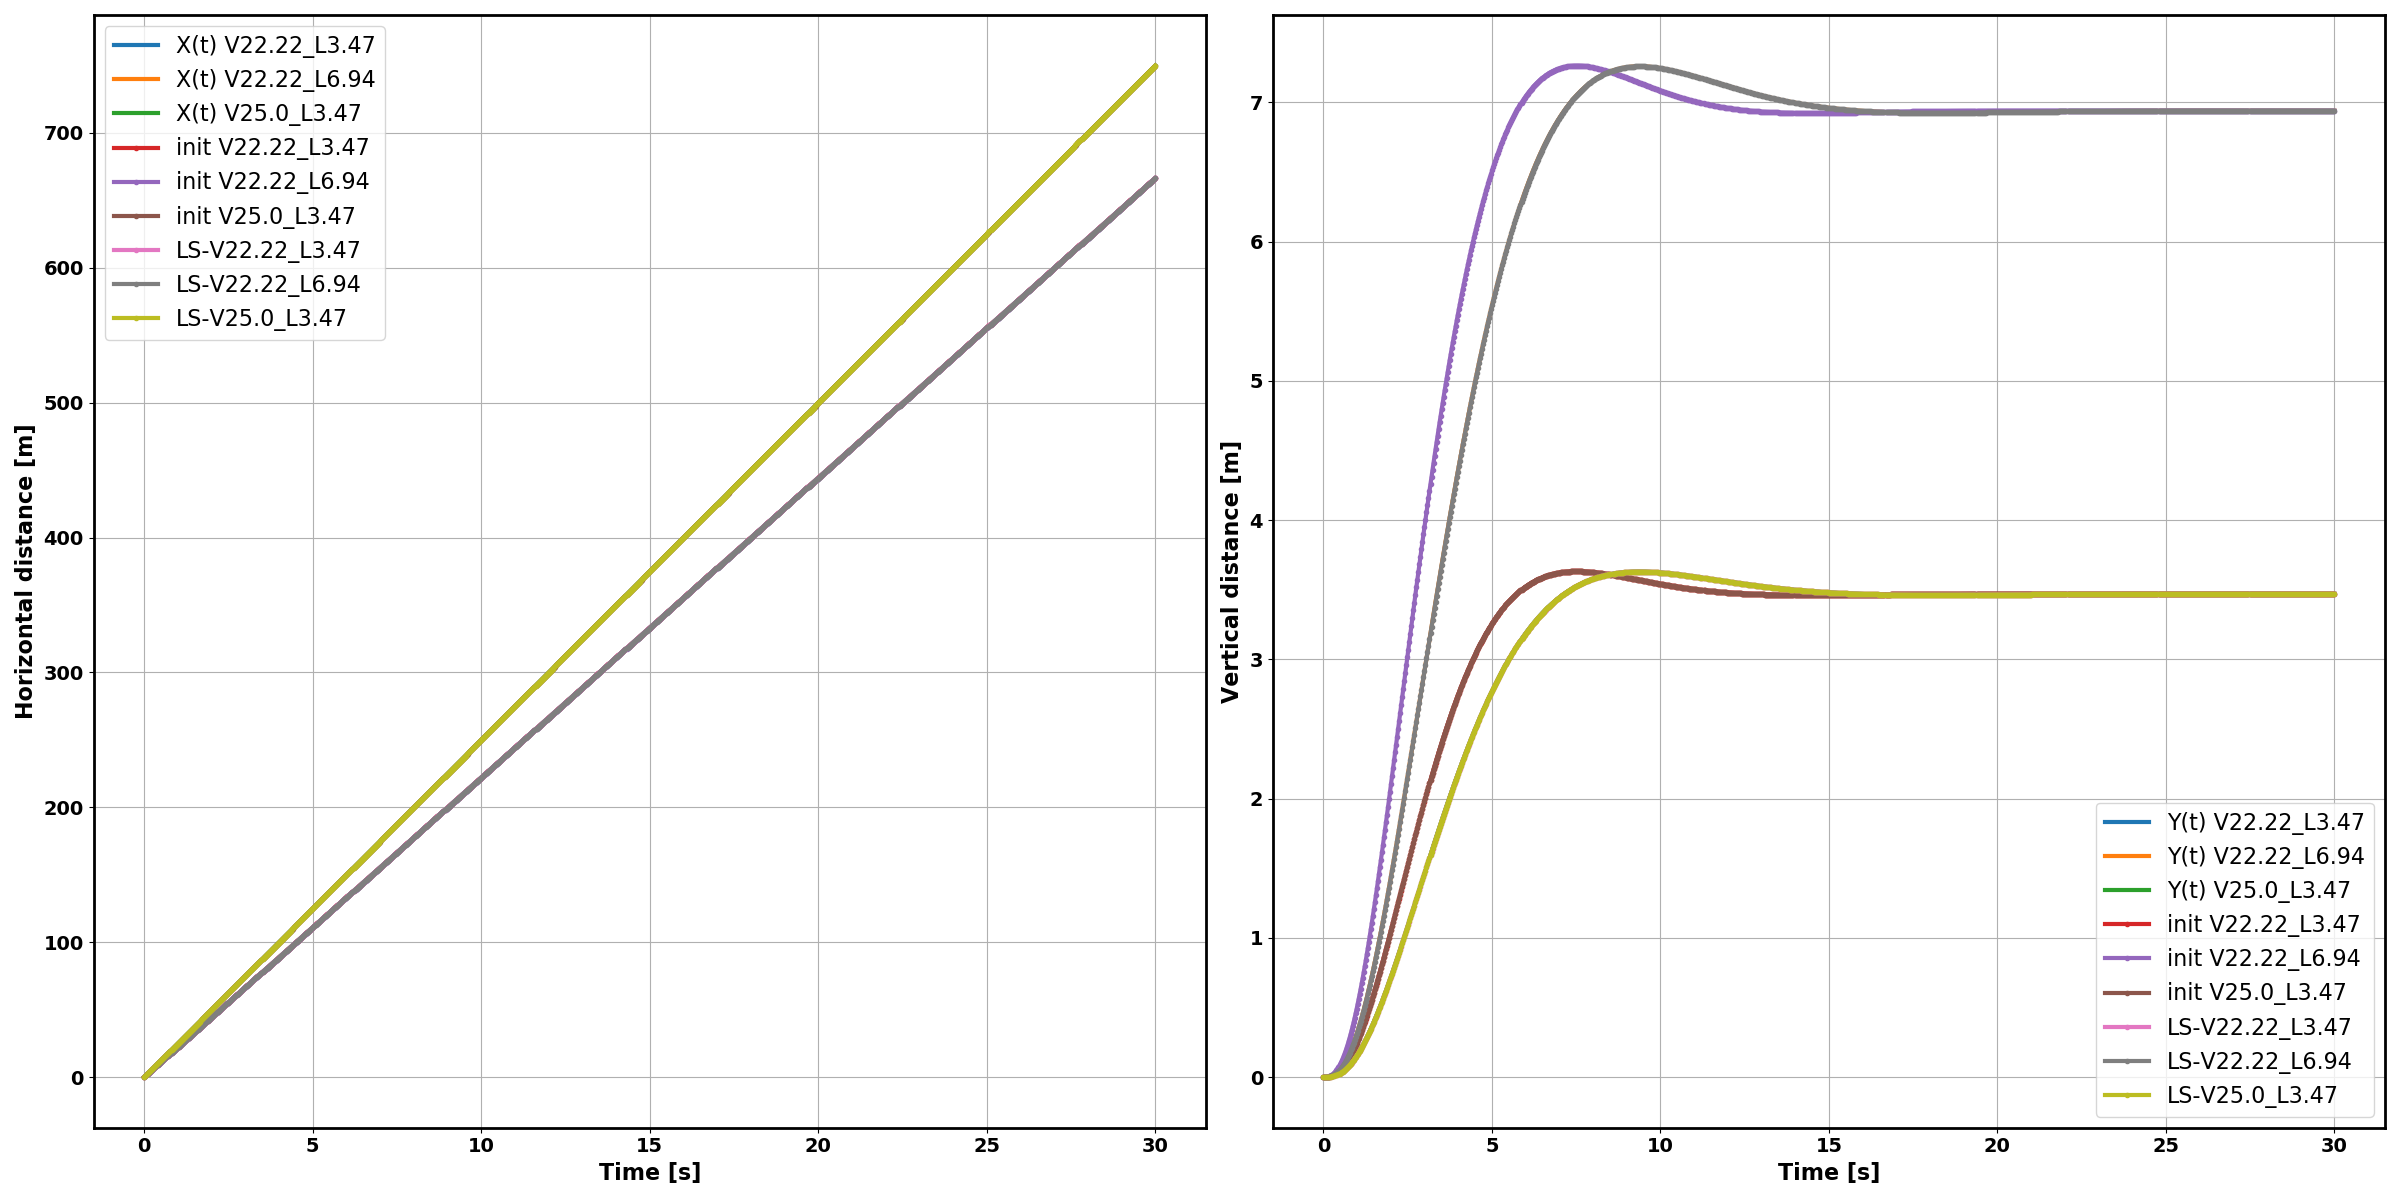
\includegraphics[width=1.0\textwidth]{1l.png}
\end{figure}

\begin{figure}[h!]
	\centering
	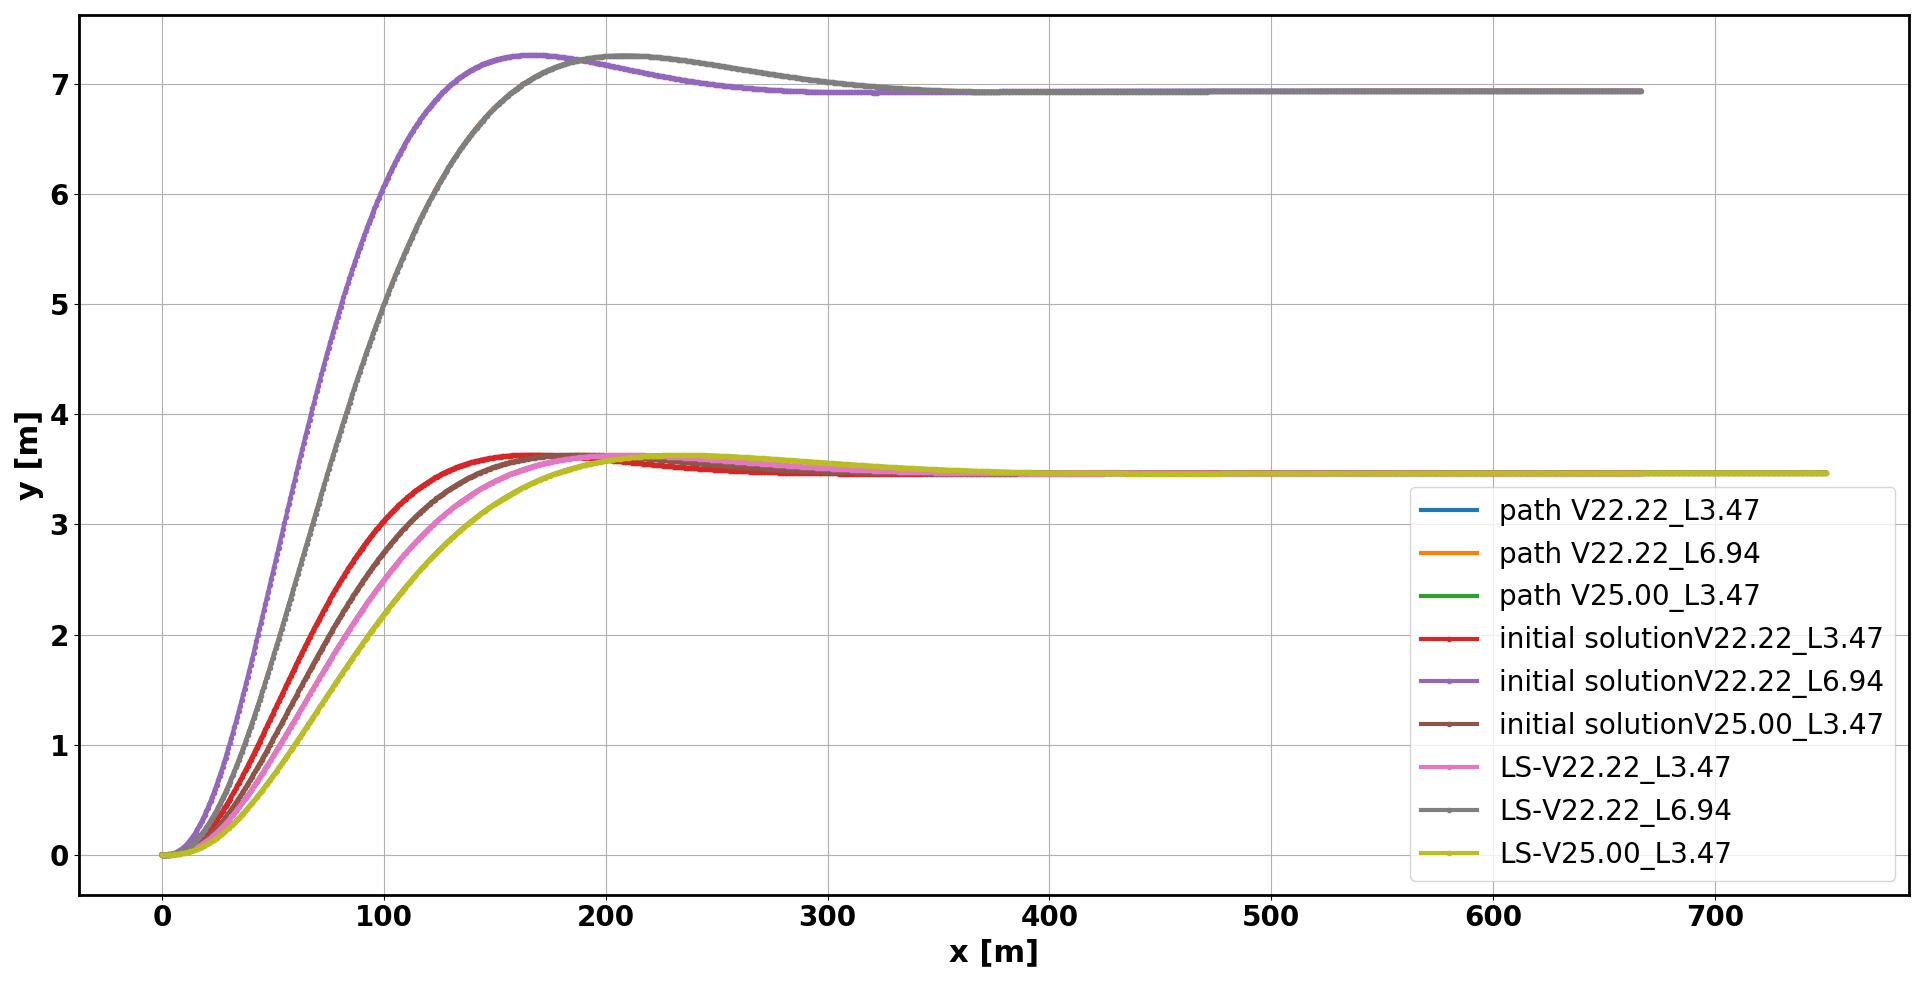
\includegraphics[width=1.0\textwidth]{2l.png}
	\label{fig:lat_acc_val}
\end{figure}

\begin{figure}[h!]
	\centering
	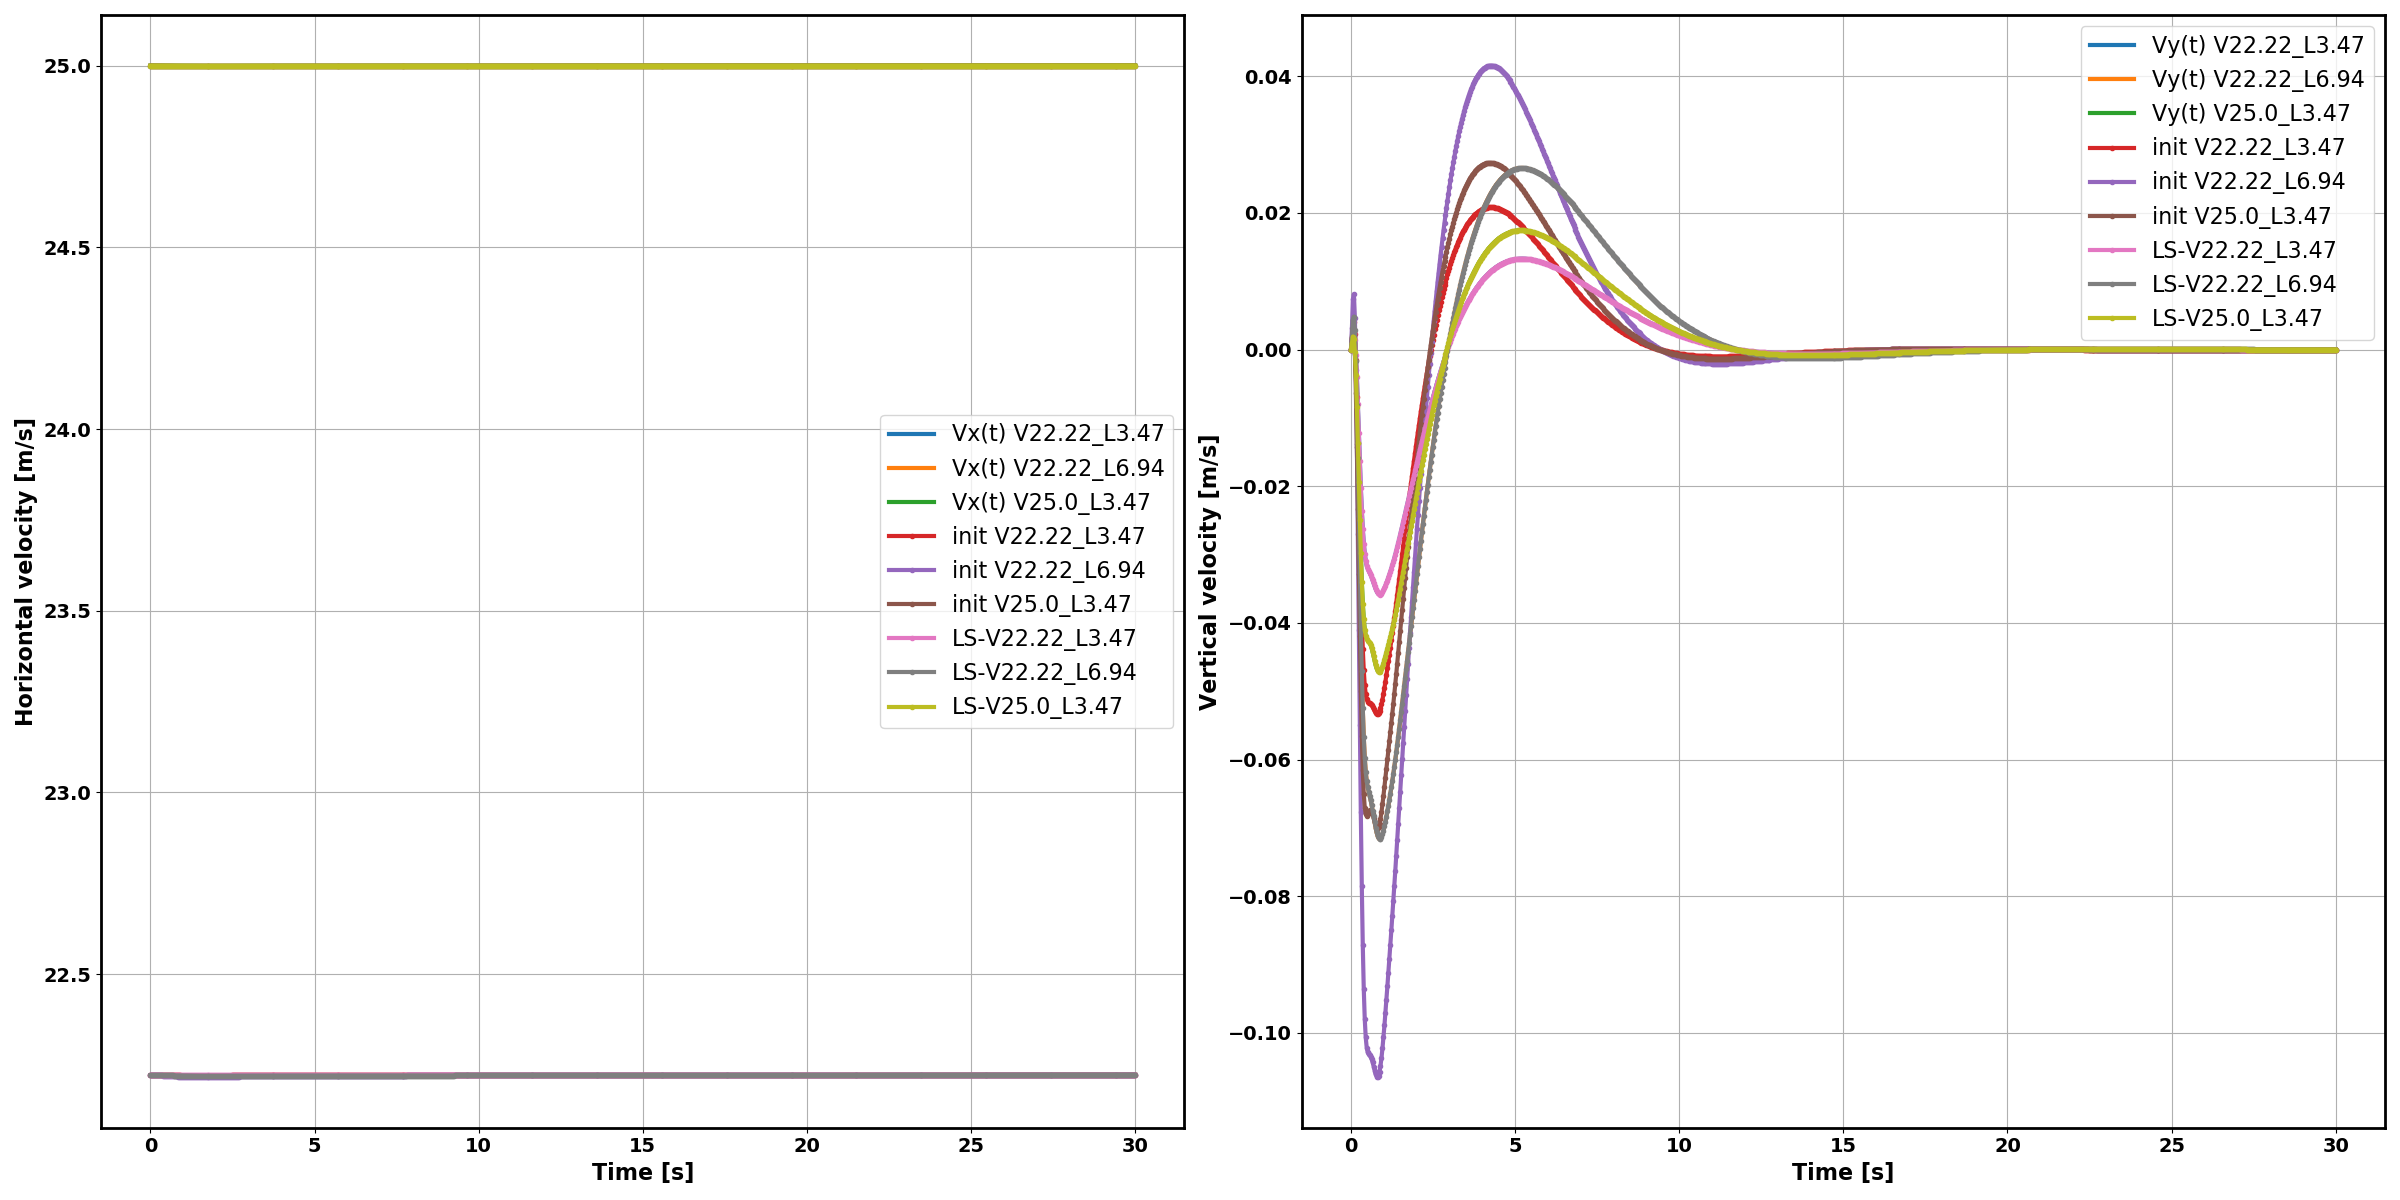
\includegraphics[width=1.0\textwidth]{3l.png}
	\label{fig:lat_acc_val}
\end{figure}


\begin{figure}[h!]
	\centering
	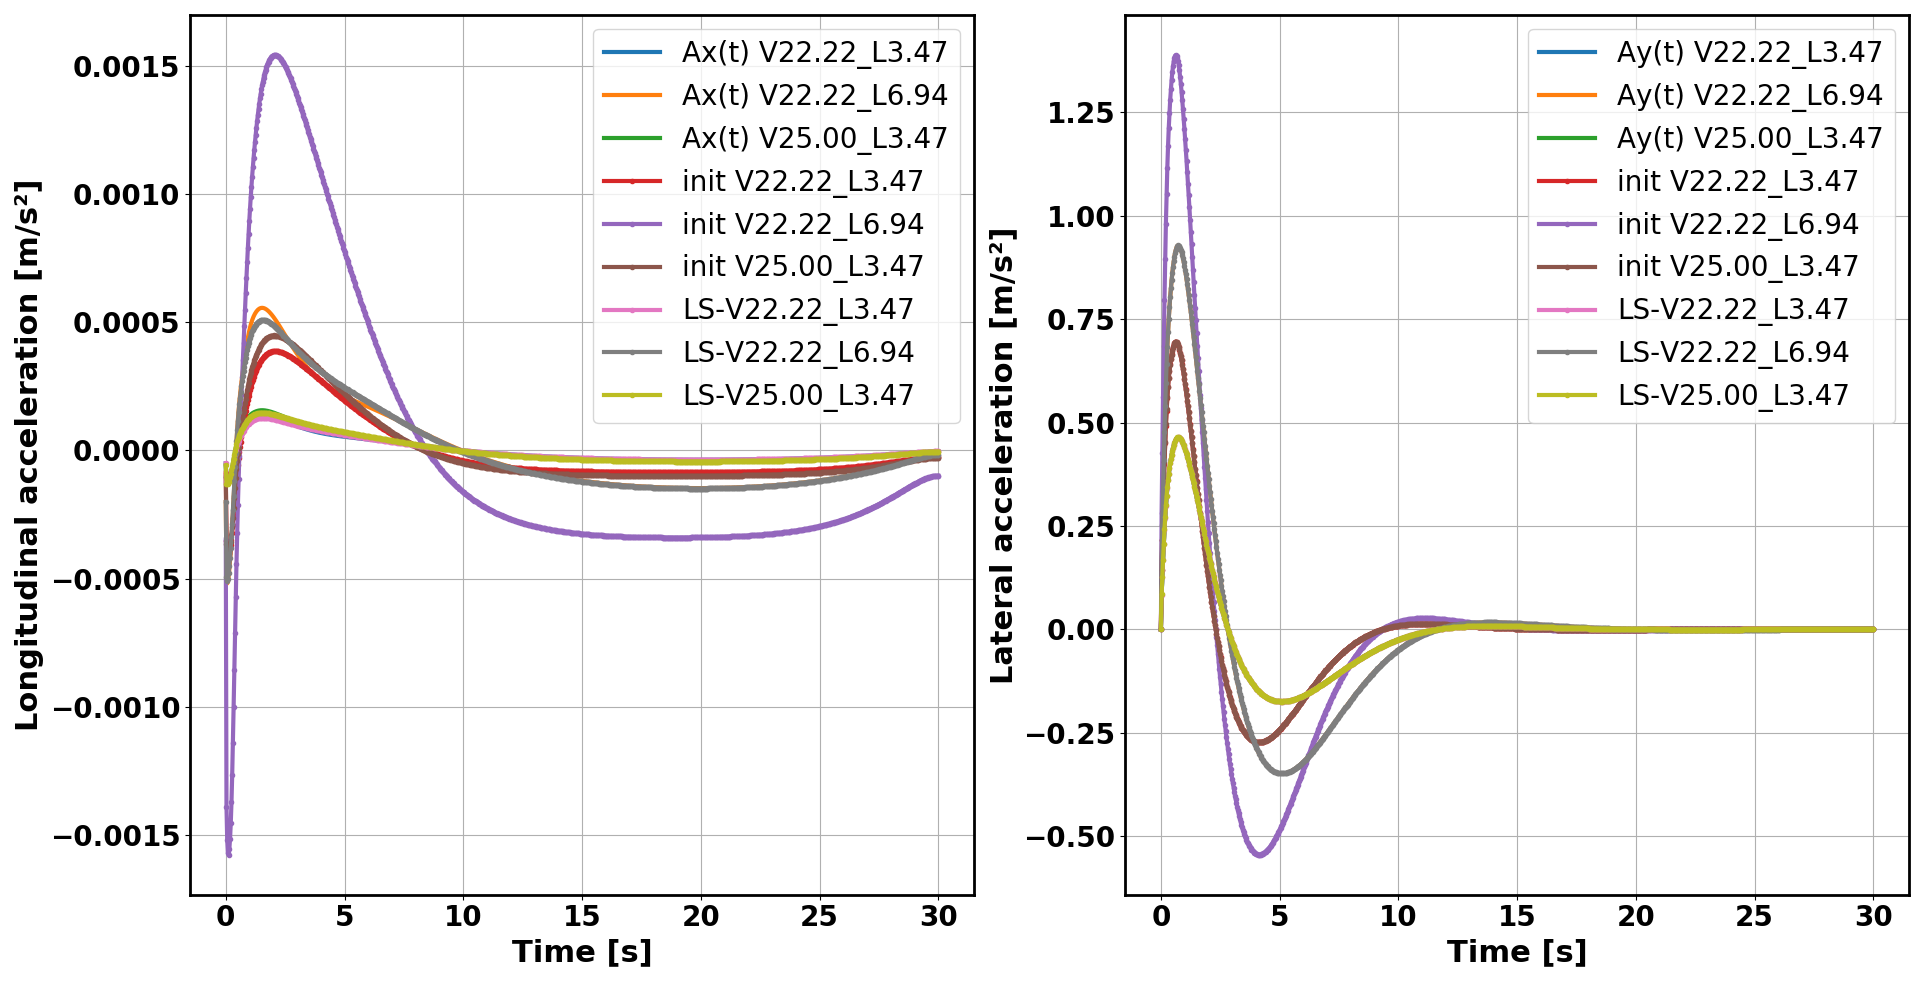
\includegraphics[width=1.0\textwidth]{4l.png}
	\label{fig:lat_acc_val}
\end{figure}


\begin{figure}[h!]
	\centering
	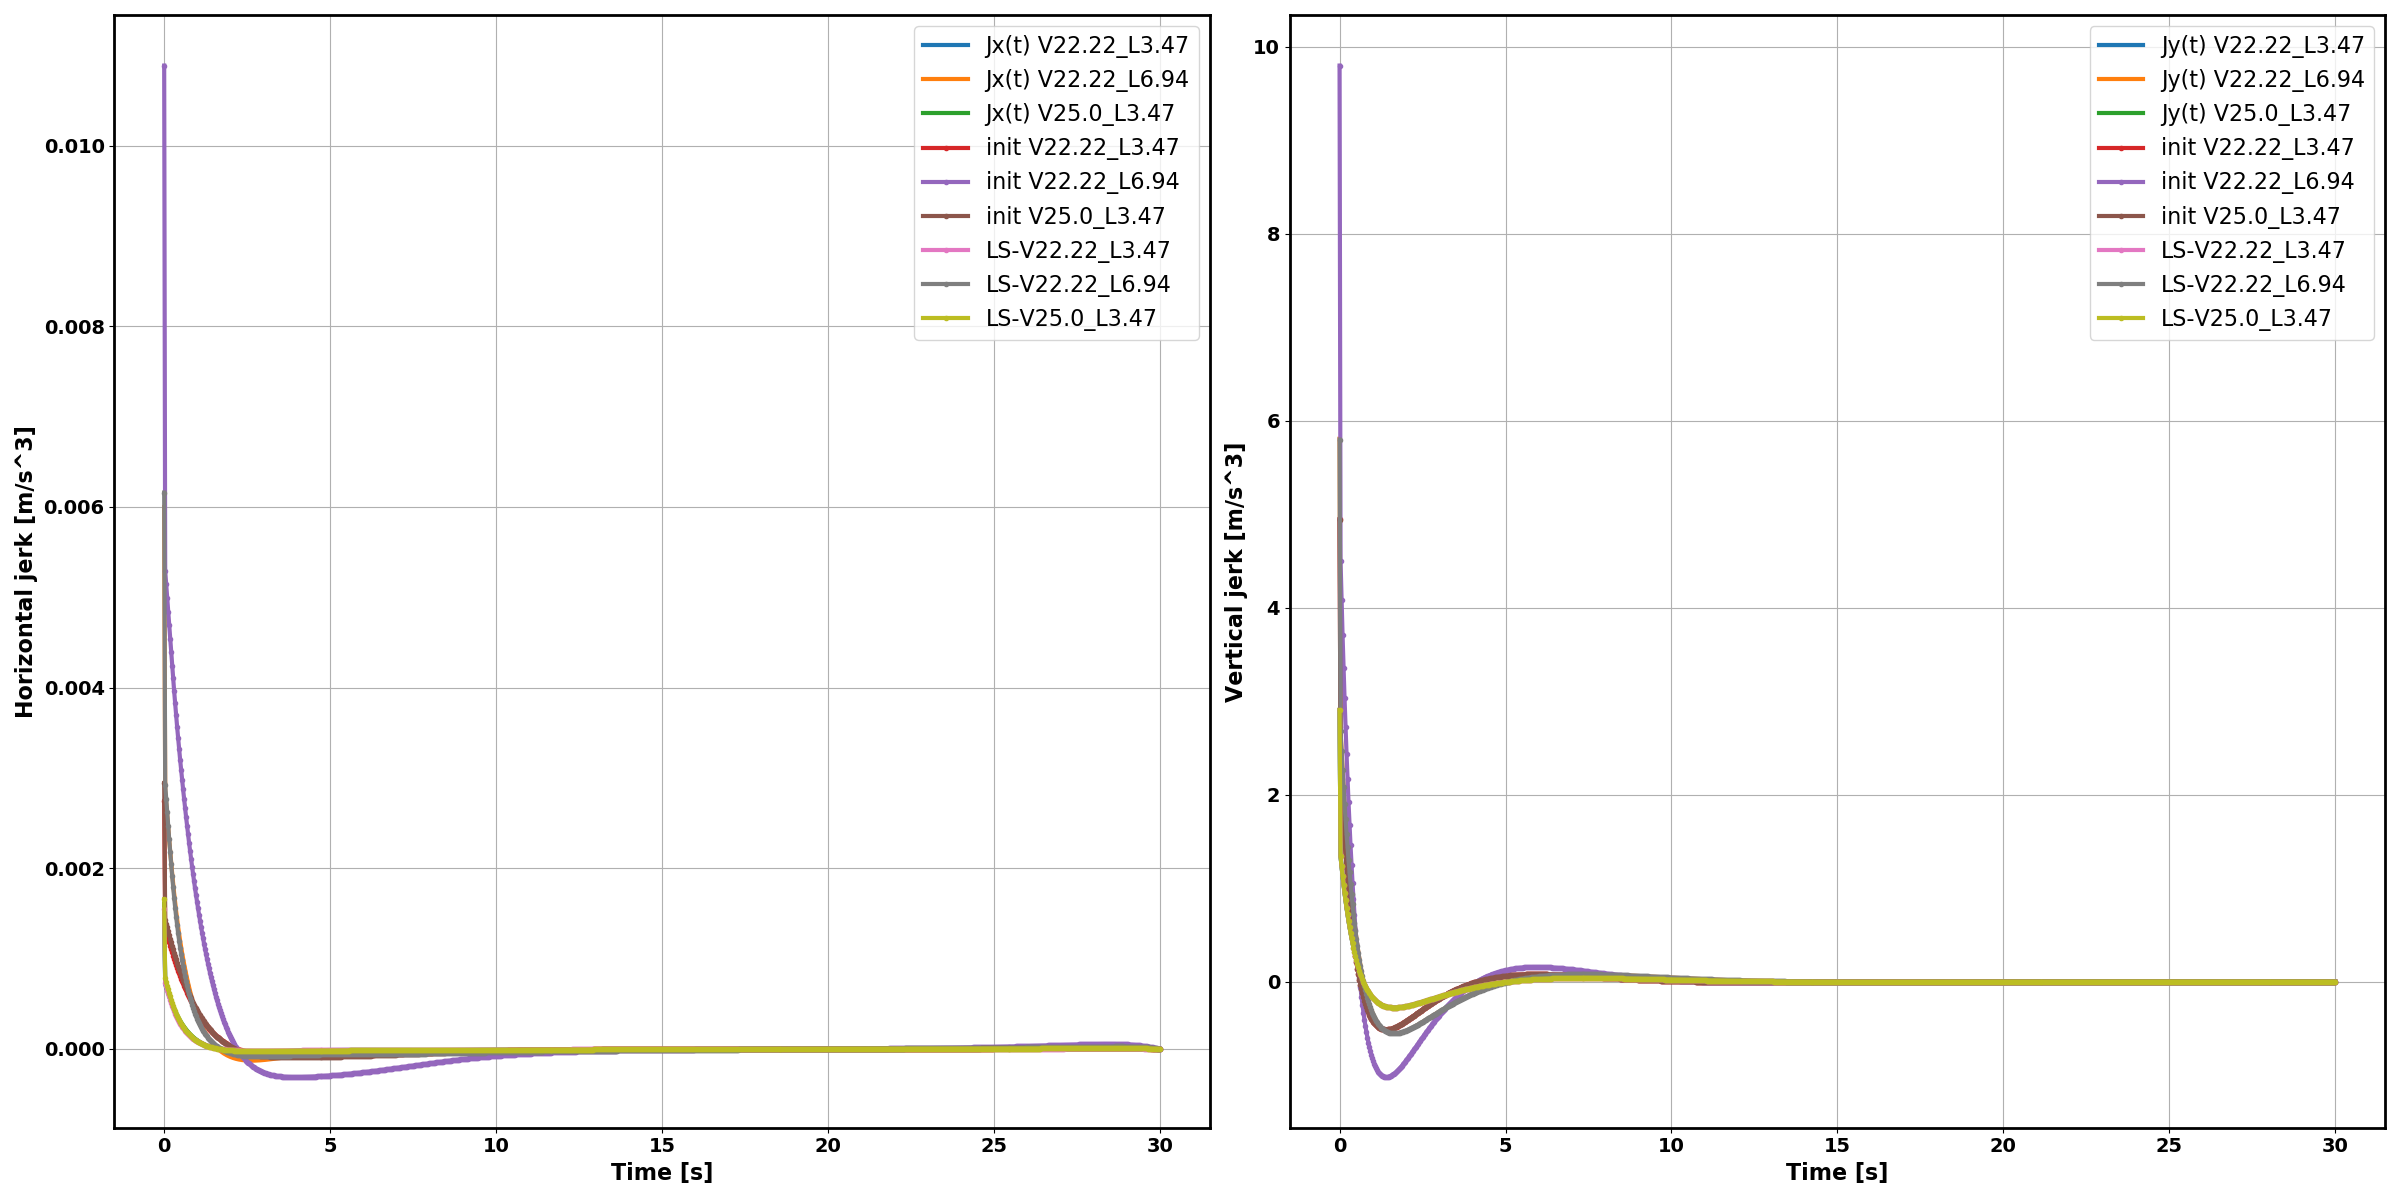
\includegraphics[width=1.0\textwidth]{5l.png}
	\label{fig:lat_acc_val}
\end{figure}


\begin{figure}[h!]
	\centering
	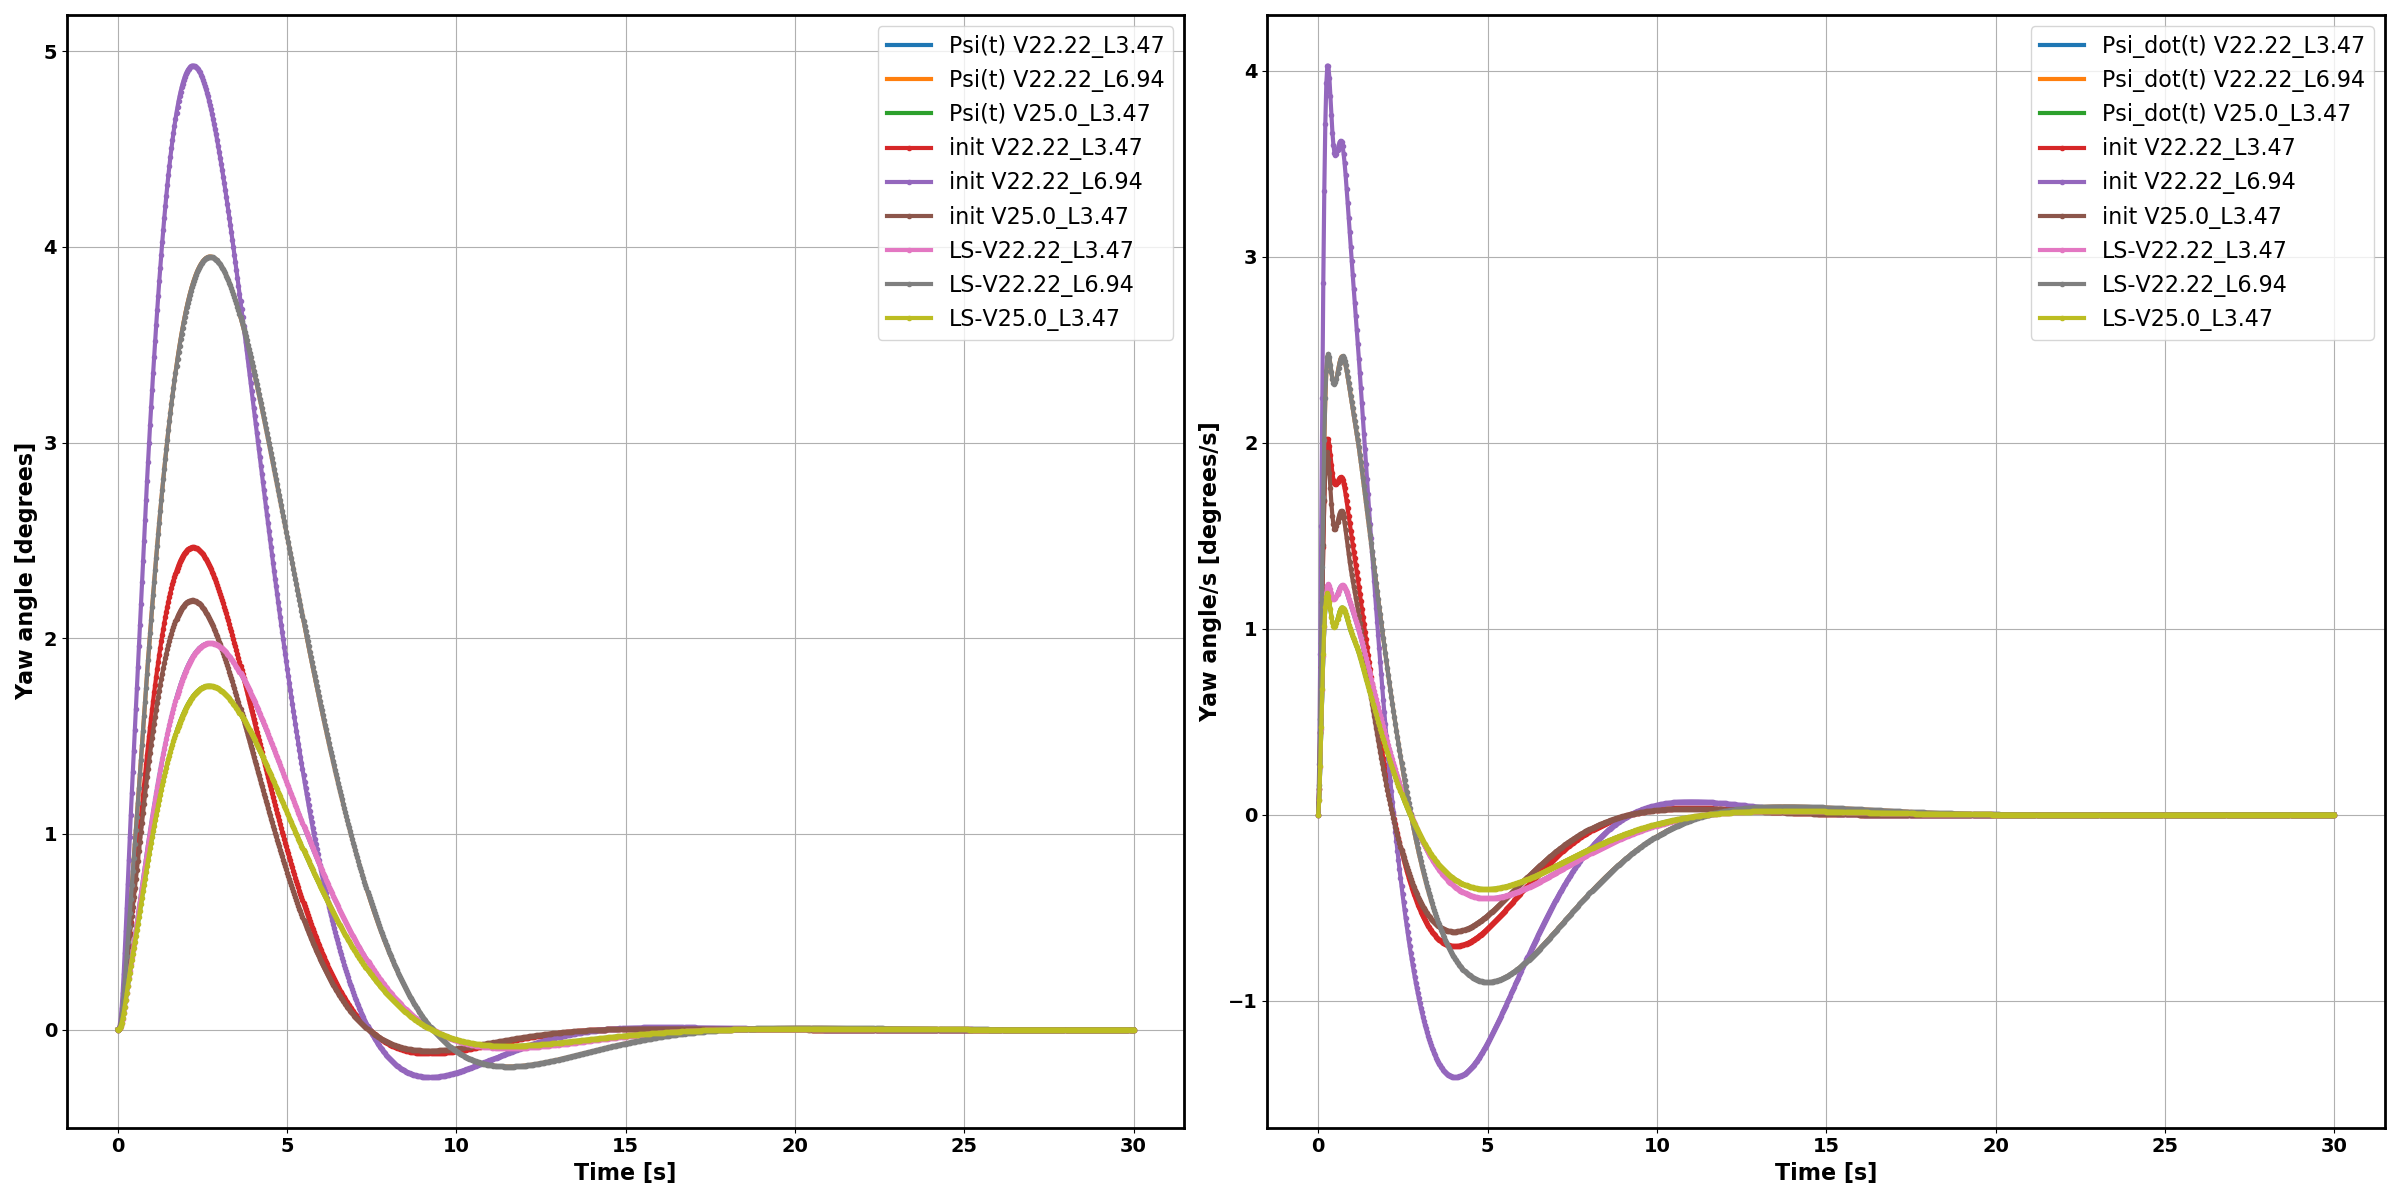
\includegraphics[width=1.0\textwidth]{6l.png}
	\label{fig:lat_acc_val}
\end{figure}


\begin{figure}[h!]
	\centering
	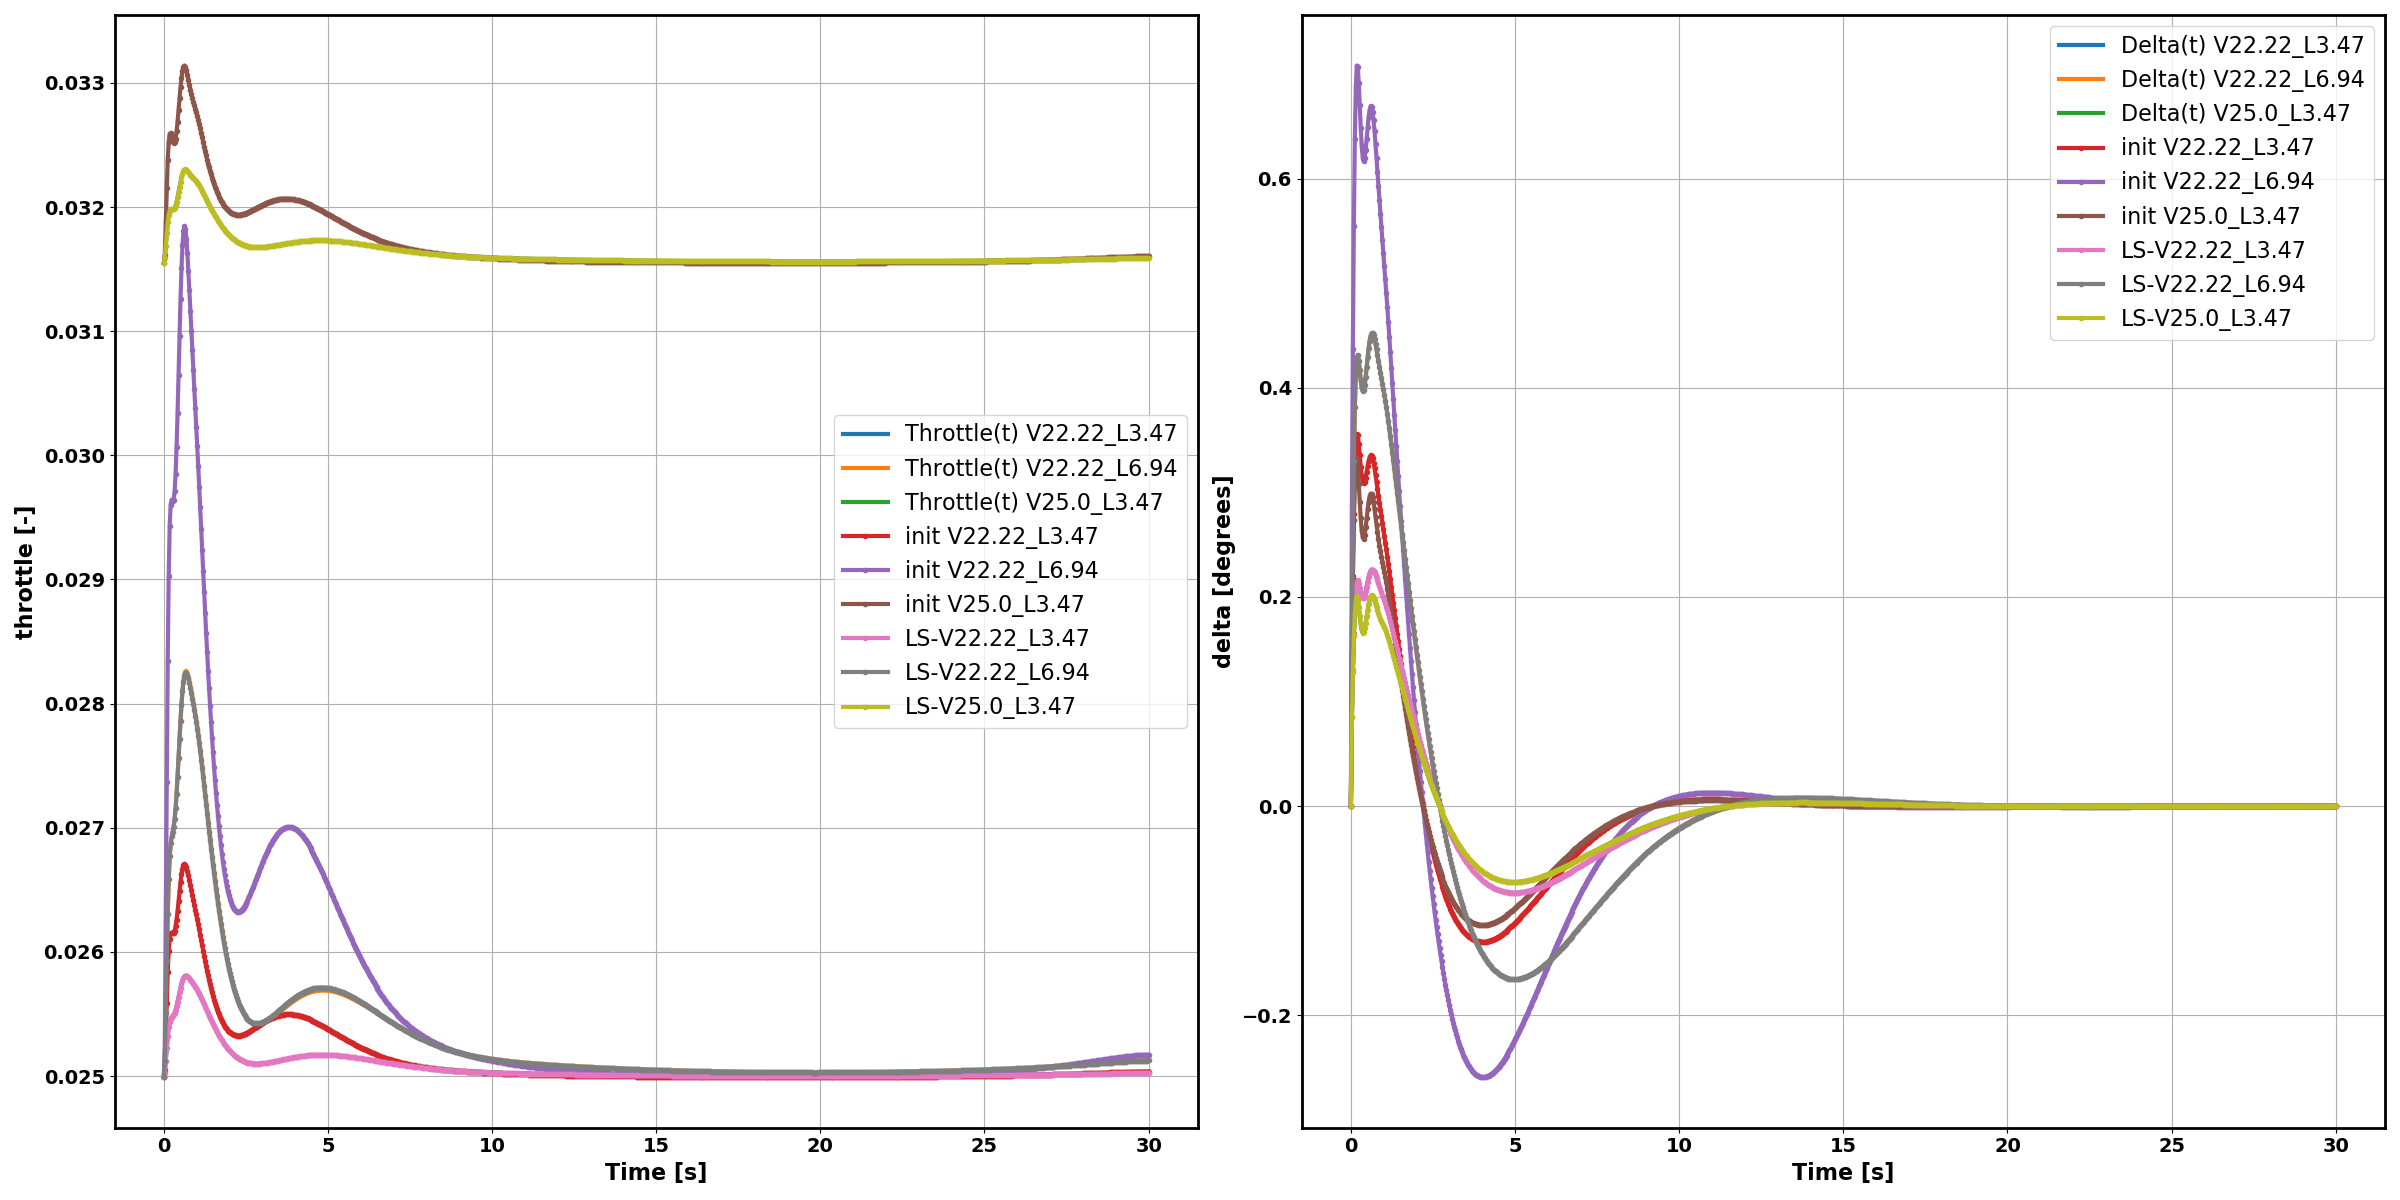
\includegraphics[width=1.0\textwidth]{7l.png}
	\caption{This figure shows the amount of throttle and the angle of the front wheel of the bicycle model during the lane change maneuvers.}
	\label{fig:app_delta}
\end{figure}


\begin{figure}[h!]
	\centering
	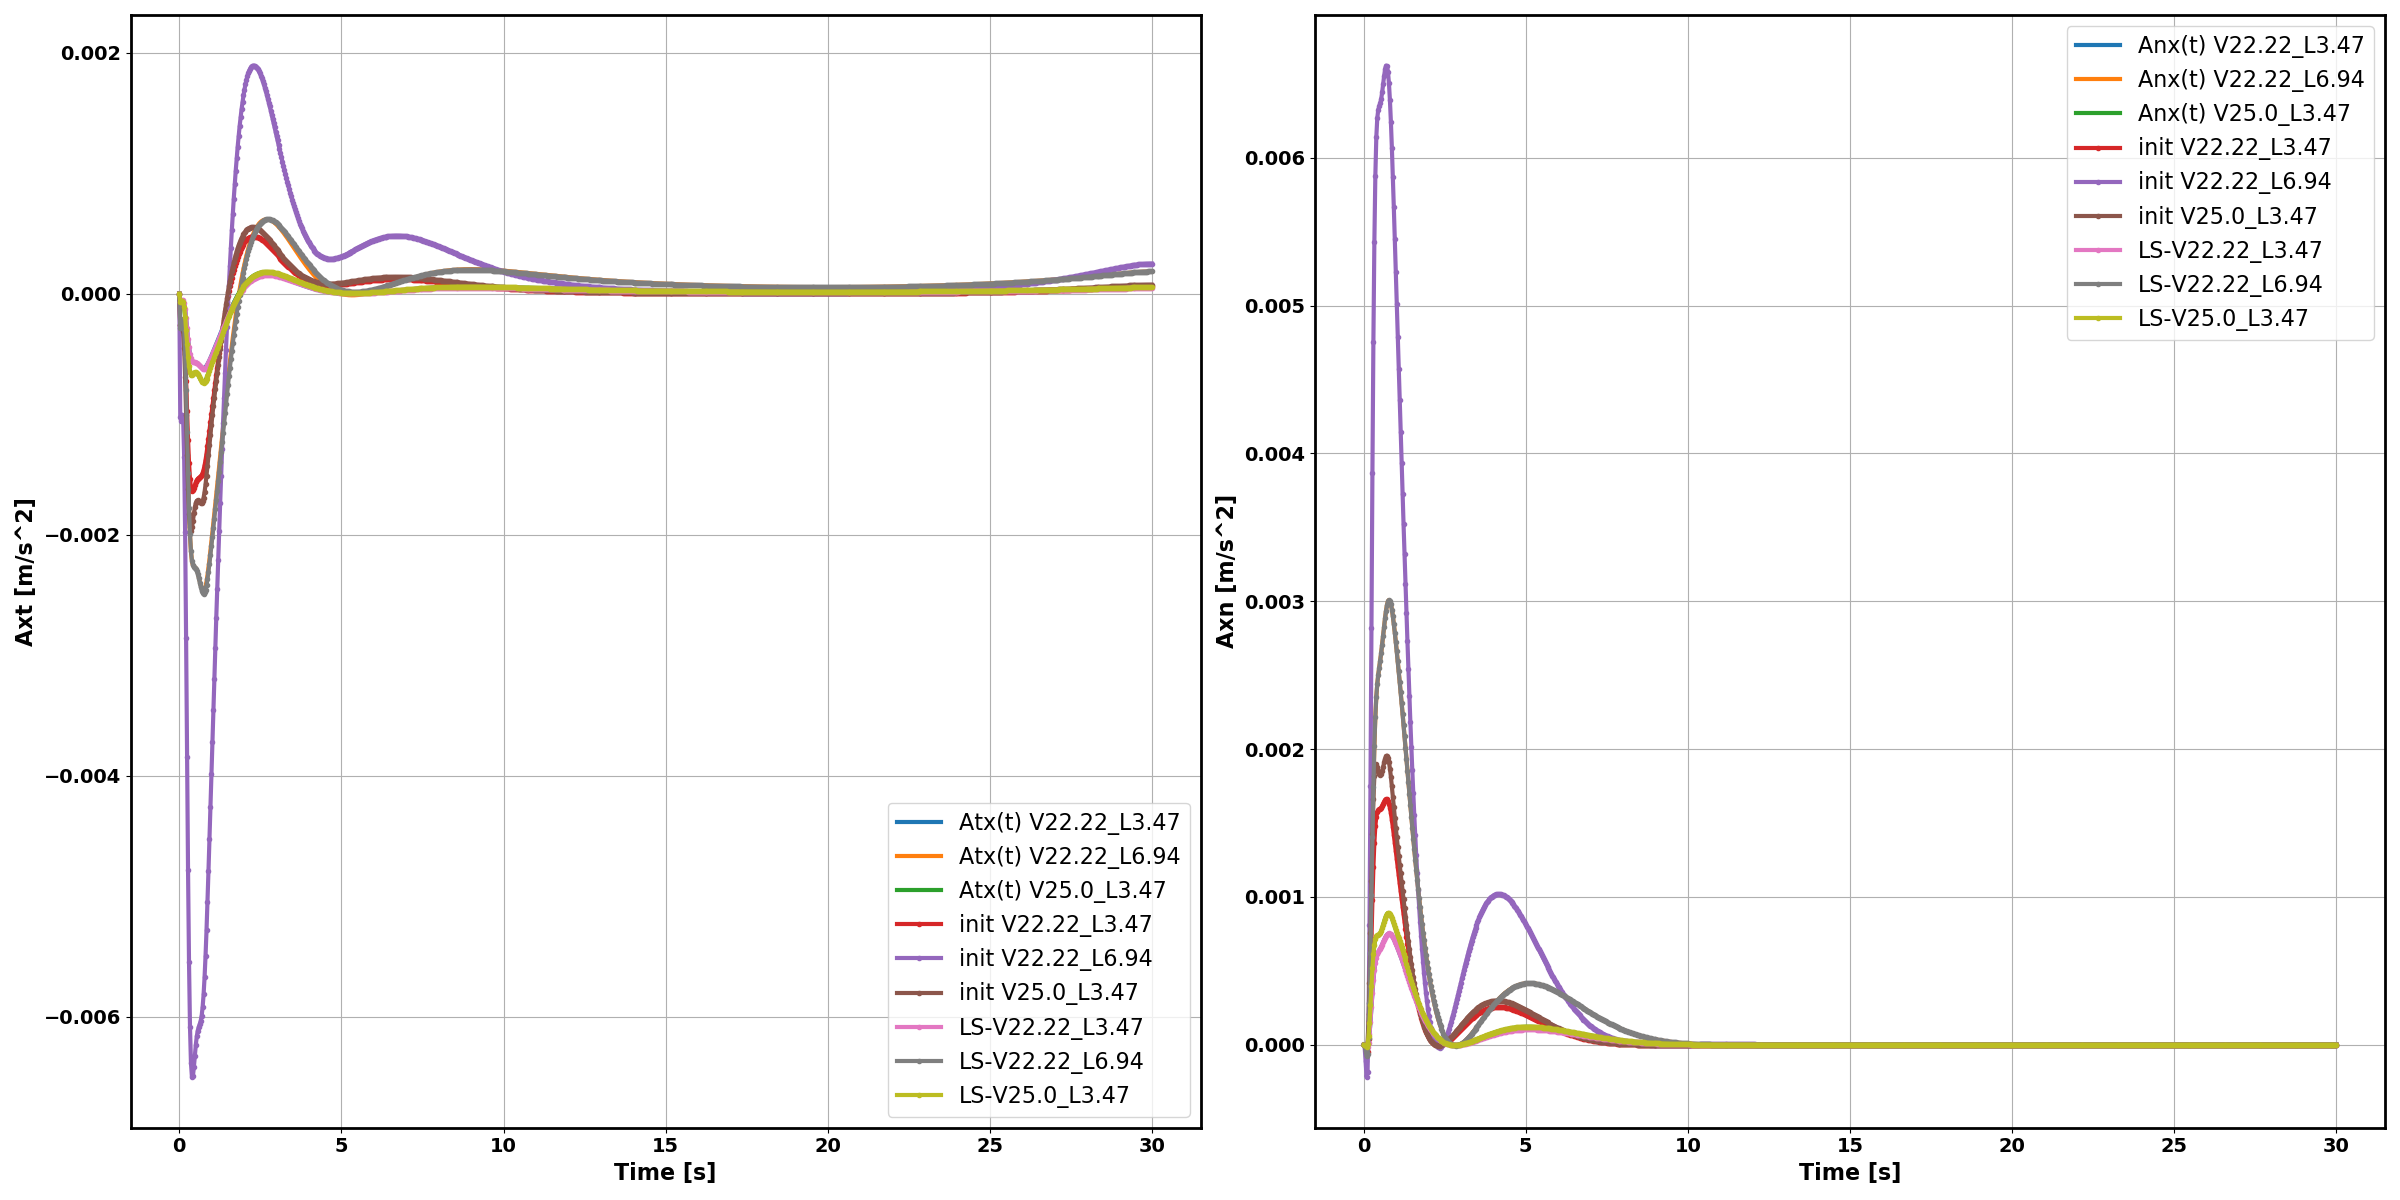
\includegraphics[width=1.0\textwidth]{8l.png}
	\label{fig:lat_acc_val}
\end{figure}


\begin{figure}[h!]
	\centering
	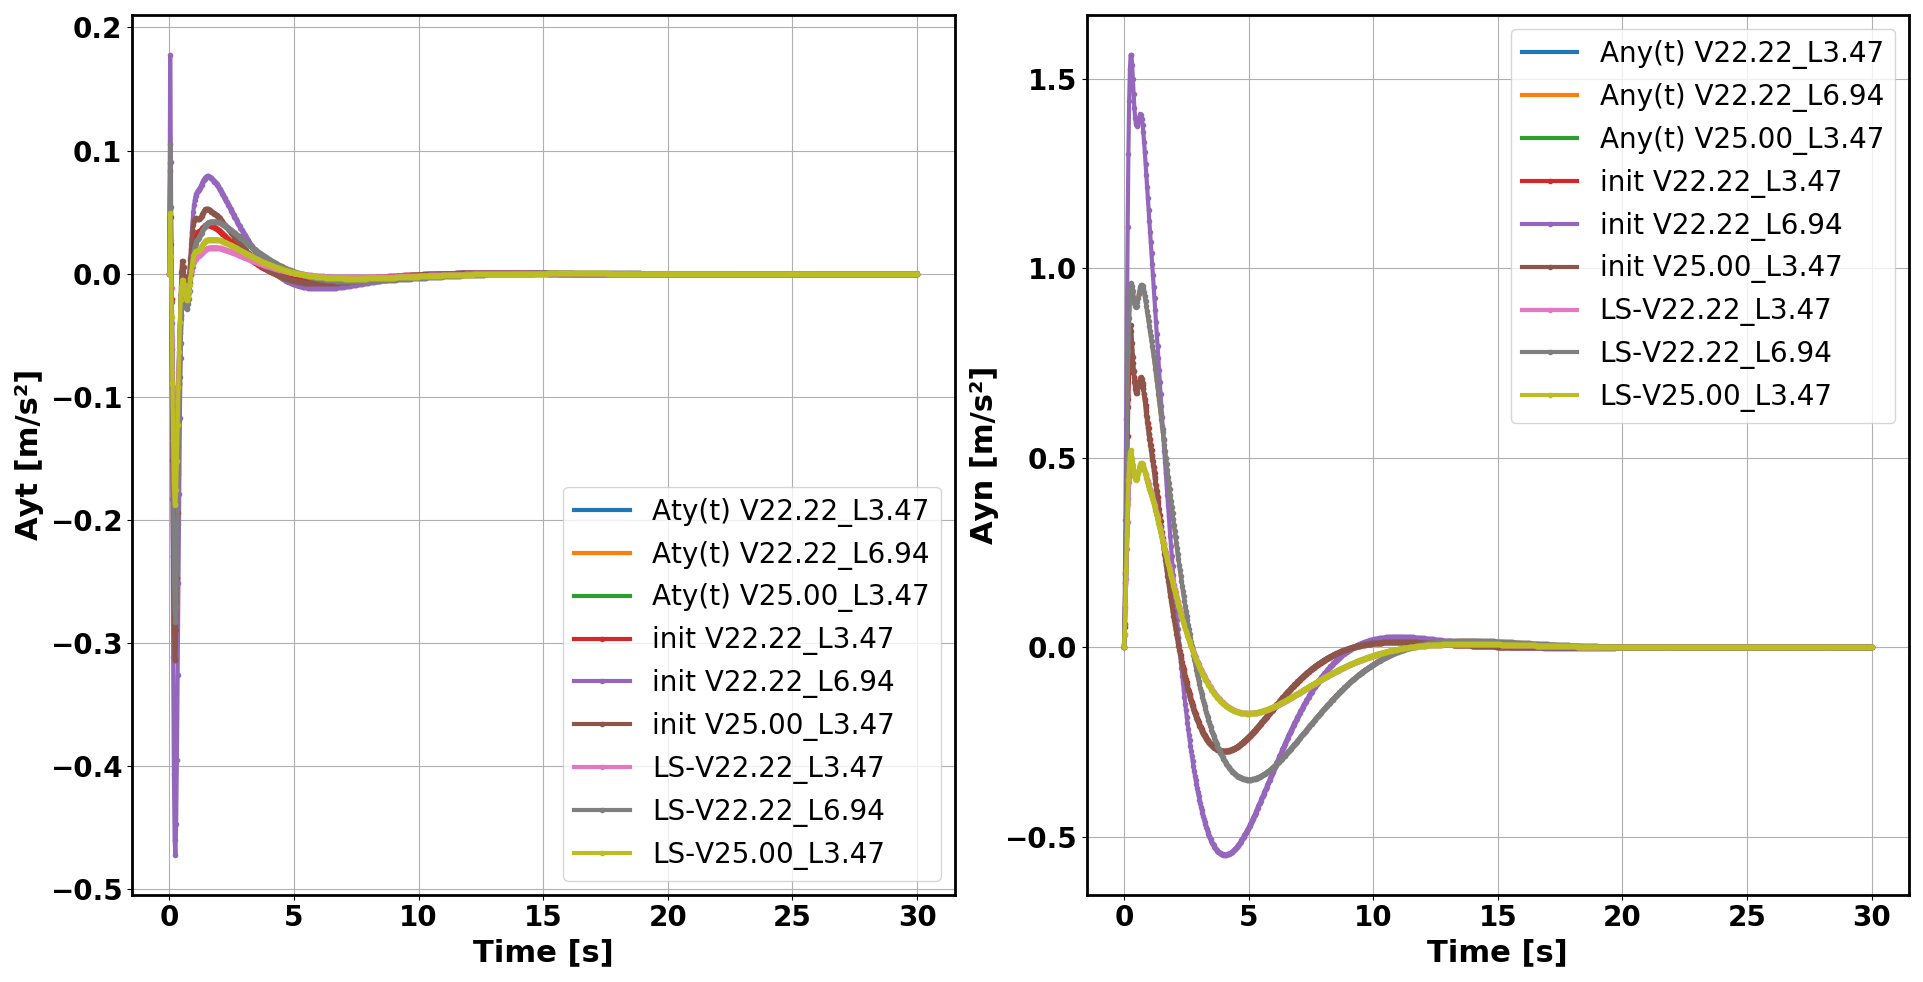
\includegraphics[width=1.0\textwidth]{9l.png}
	\label{fig:lat_acc_val}
\end{figure}


\begin{figure}[h!]
	\centering
	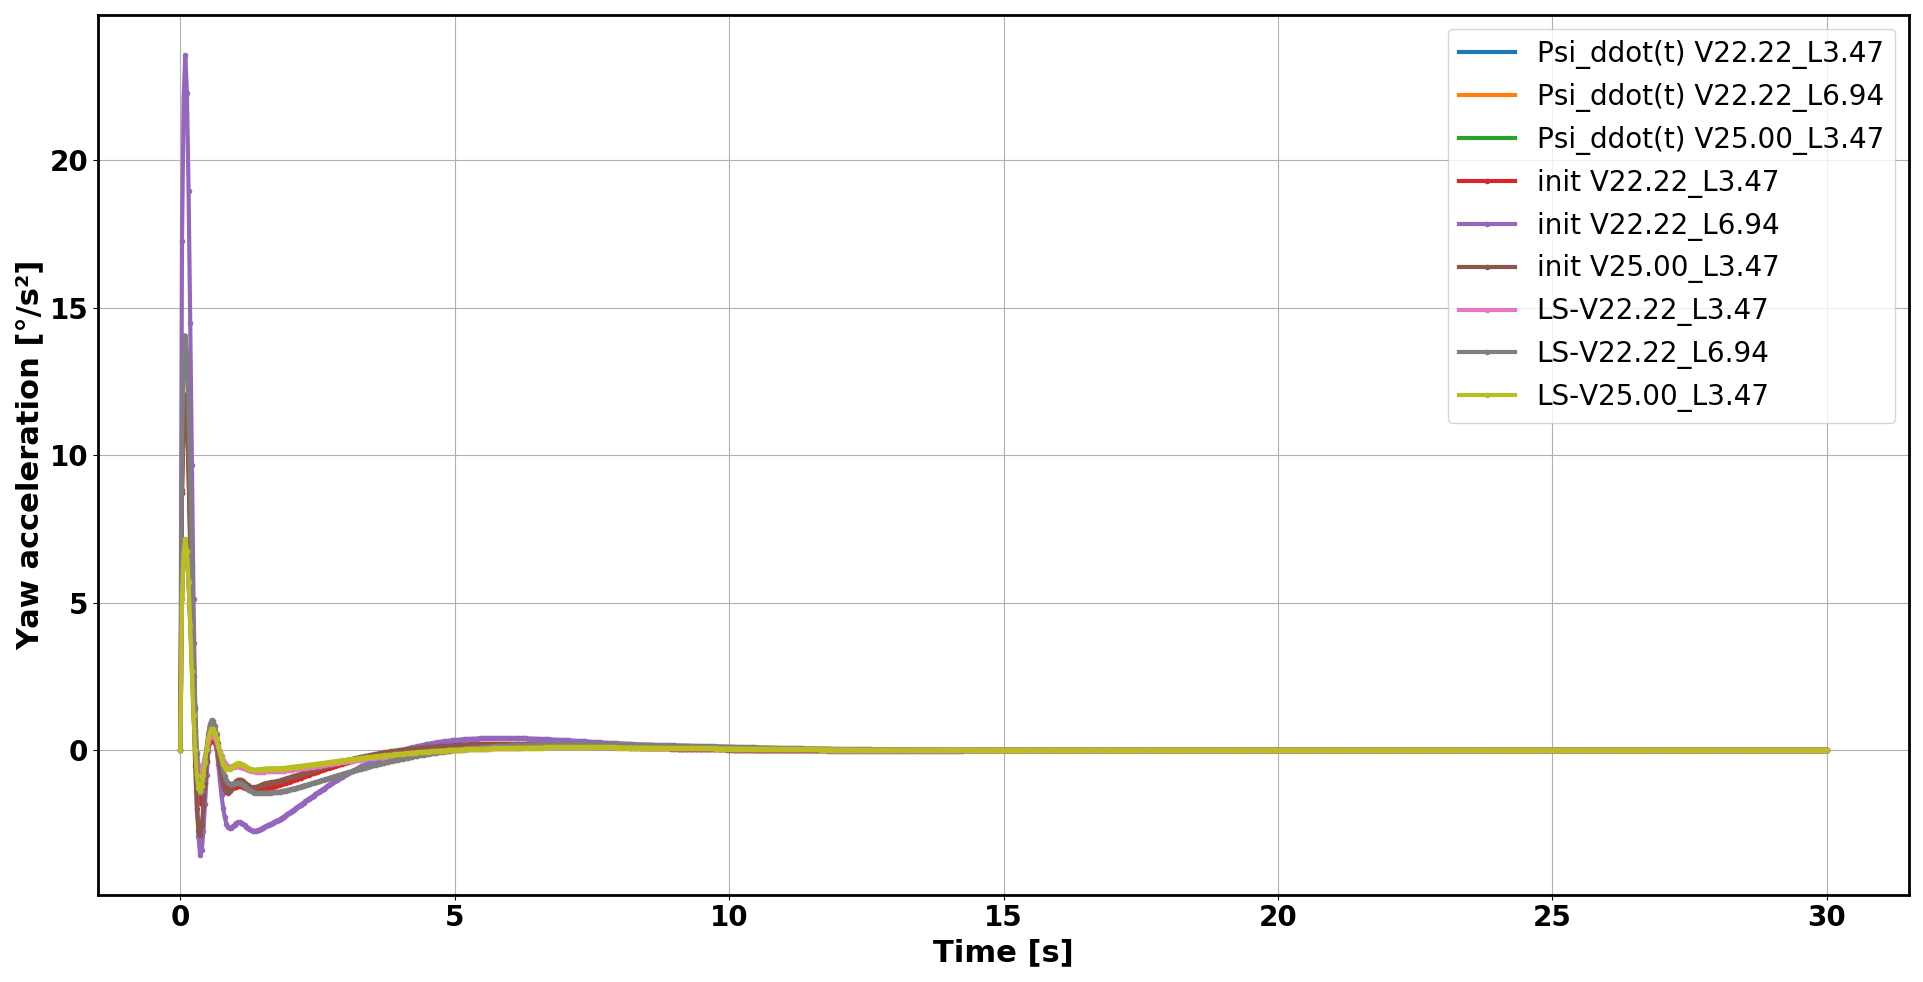
\includegraphics[width=1.0\textwidth]{10l.png}
	\label{fig:lat_acc_val}
\end{figure}


\begin{figure}[h!]
	\centering
	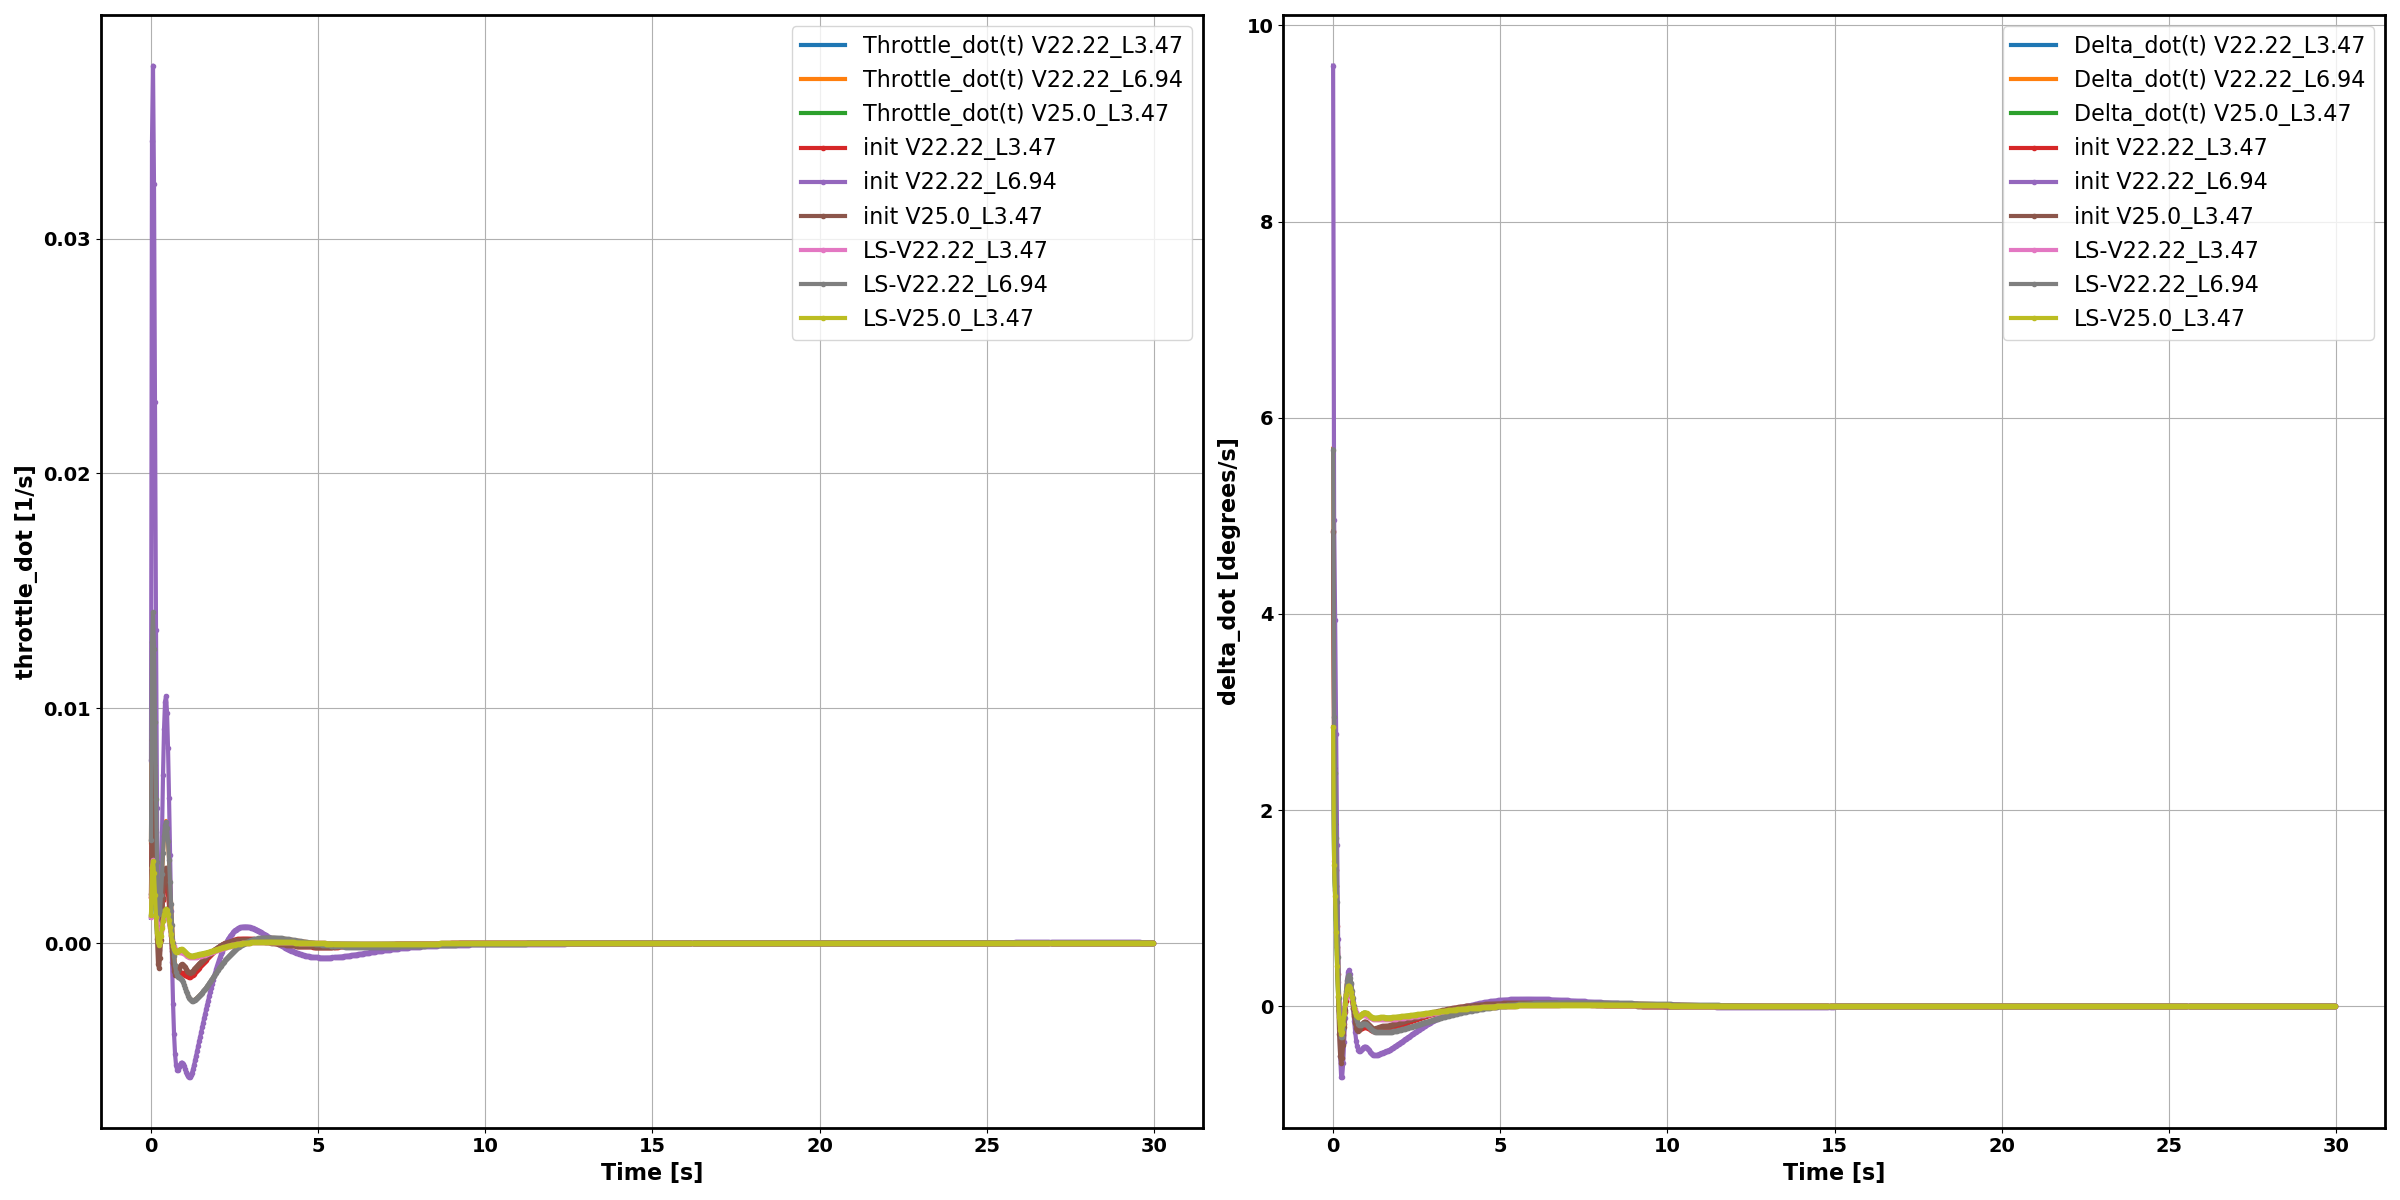
\includegraphics[width=1.0\textwidth]{11l.png}
	\caption{This figure shows the amount of first derivative of throttle and the first derivative of the angle of the front wheel of the bicycle model is given as input during the lane change maneuvers.}
	\label{fig:app_delta_dot}
\end{figure}


\begin{figure}[h!]
	\centering
	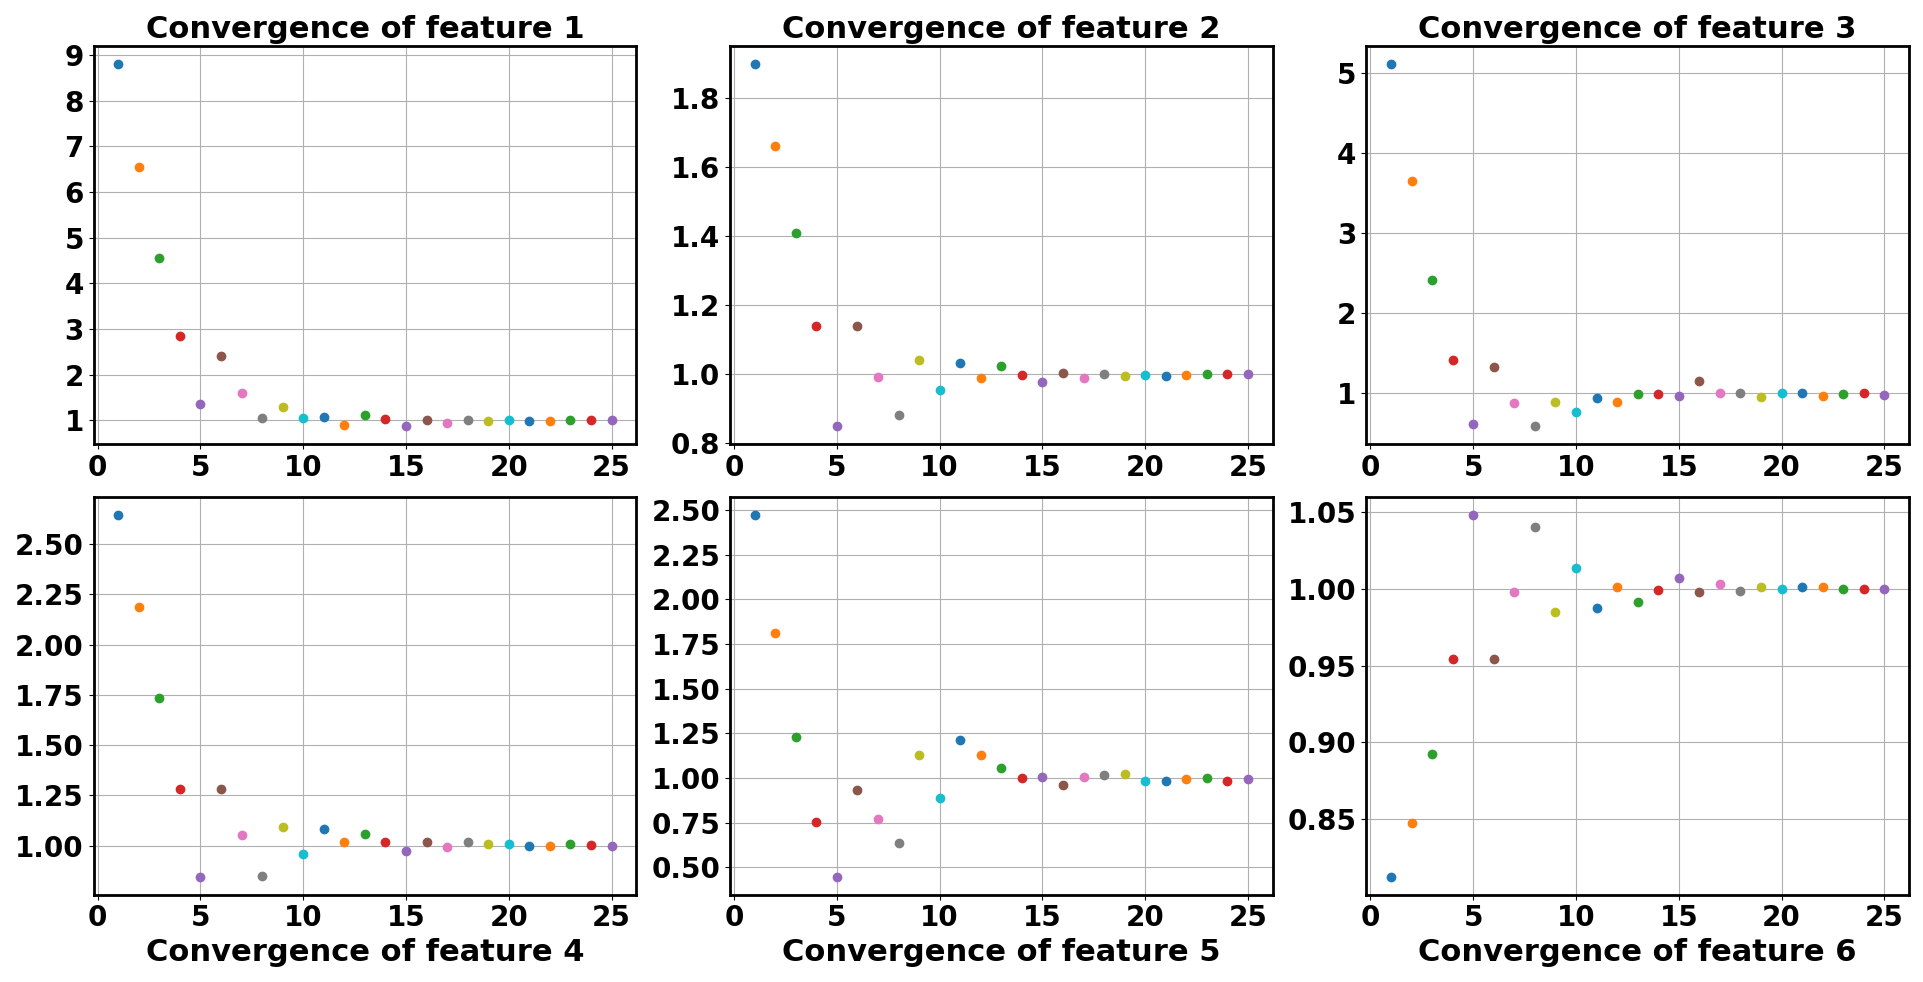
\includegraphics[width=1.0\textwidth]{12l.png}	
	\caption{The convergence of $\bm{f}_{rel}$ towards one during the learning iterations.}
	\label{fig:app_conv}
\end{figure}


\begin{figure}[h!]
	\centering
	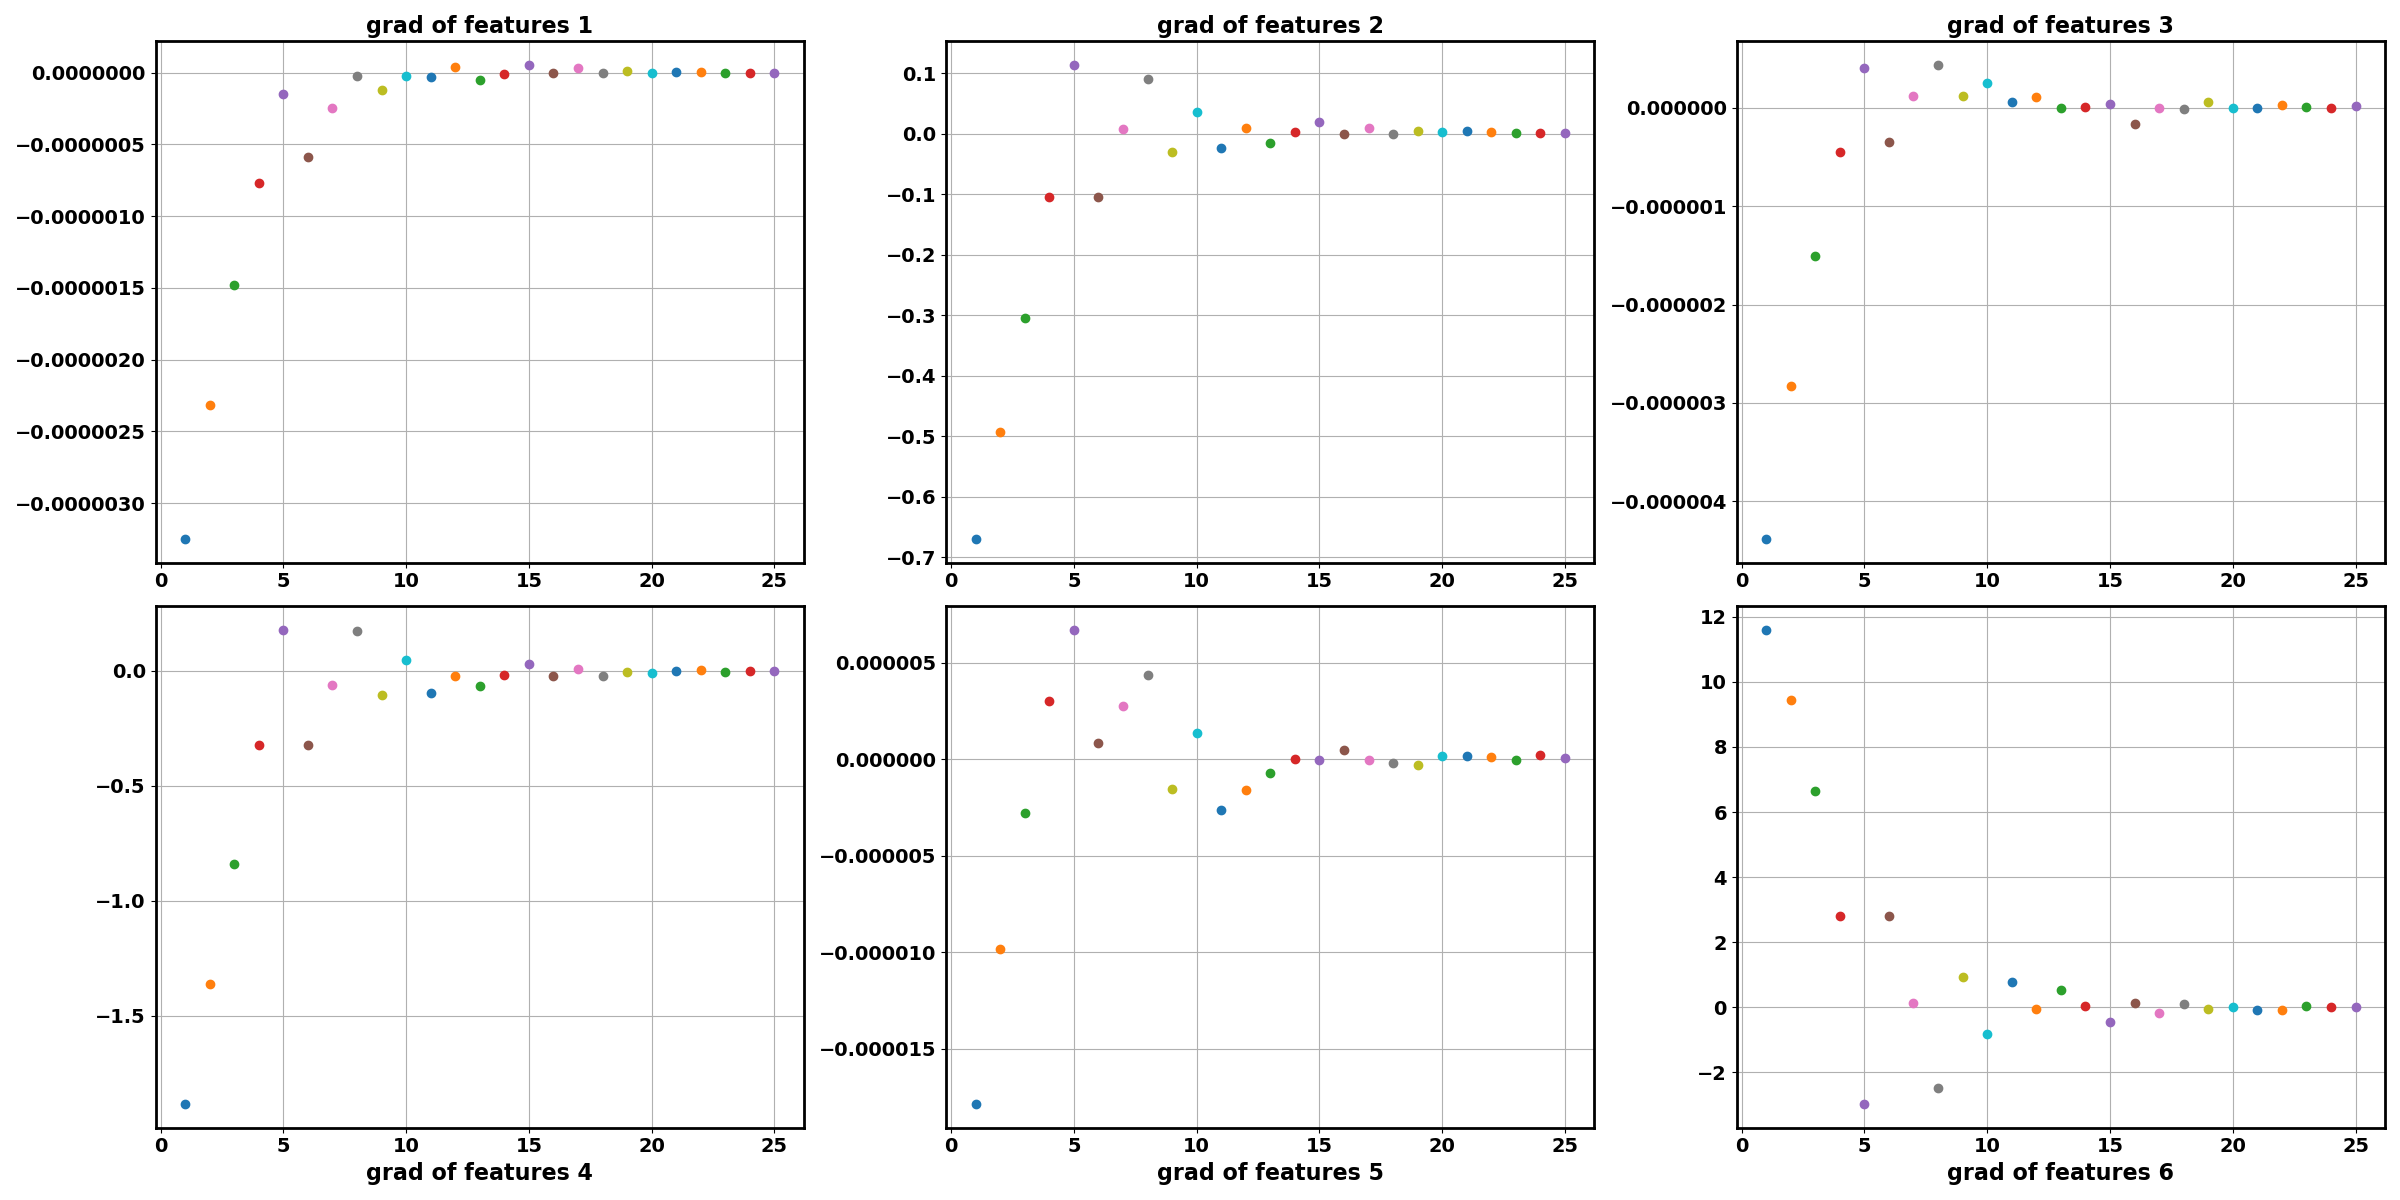
\includegraphics[width=1.0\textwidth]{13l.png}
	\caption{The gradient $\pdv{\bm{F}}{\bm{\theta}}$ estimated by $\bm{F}_{obs} - \bm{F}(\bm{r}_{expected})$ towards zero during the different learning iterations. }
	\label{fig:app_grad}
\end{figure}

\begin{figure}[h!]
	\centering
	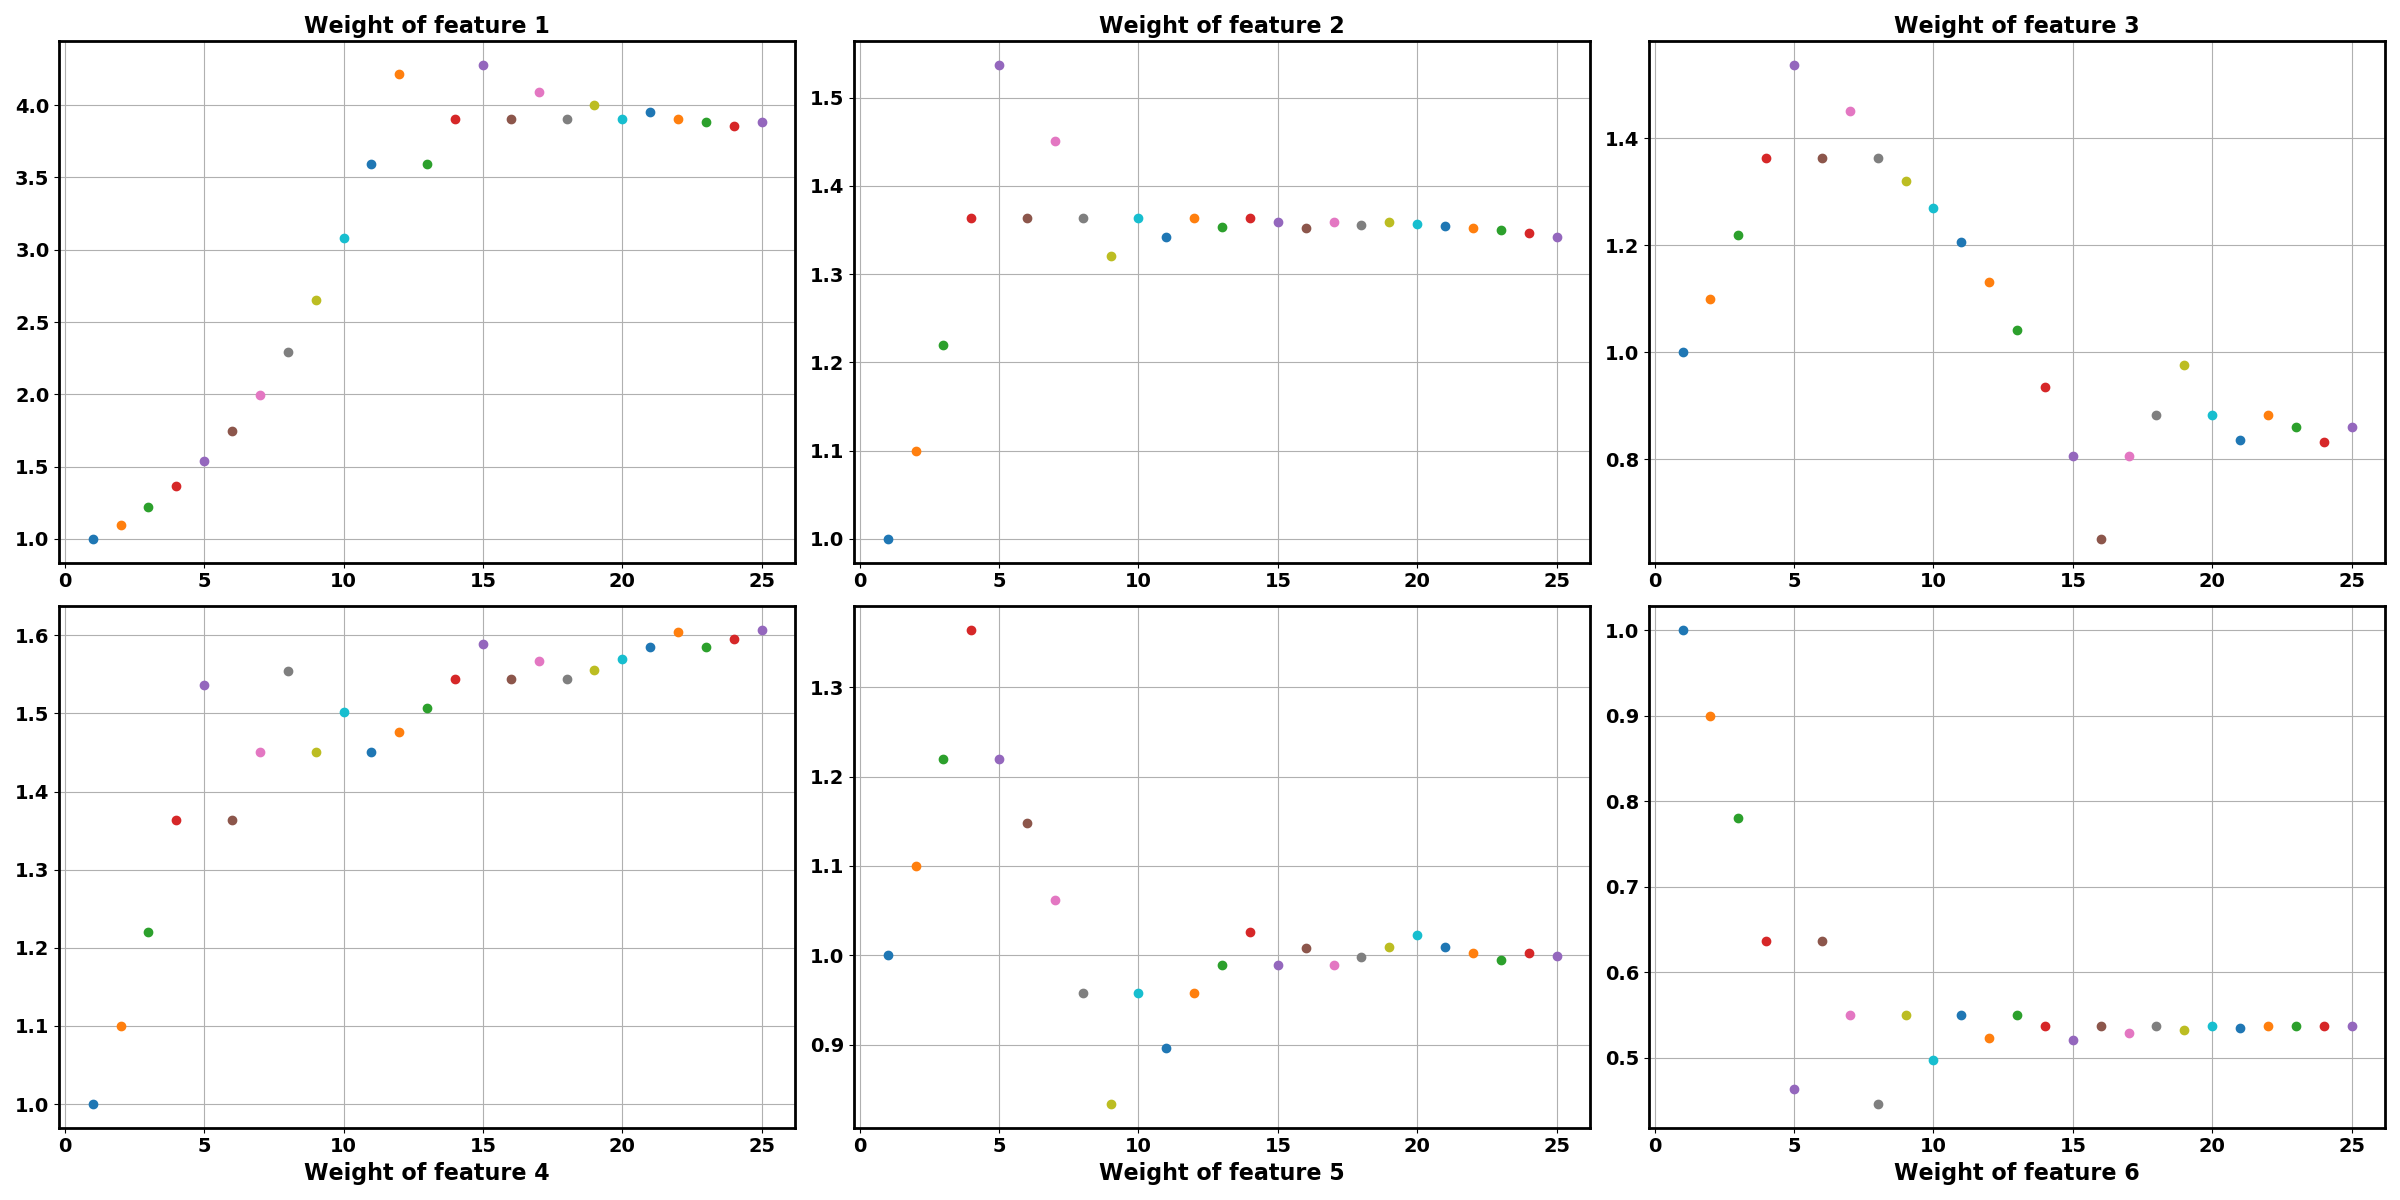
\includegraphics[width=1.0\textwidth]{14l.png}
	\caption{The learned weights during the different learning iterations.}
	\label{fig:app_weights}
	
\end{figure}


\begin{figure}[h!]
	\centering
	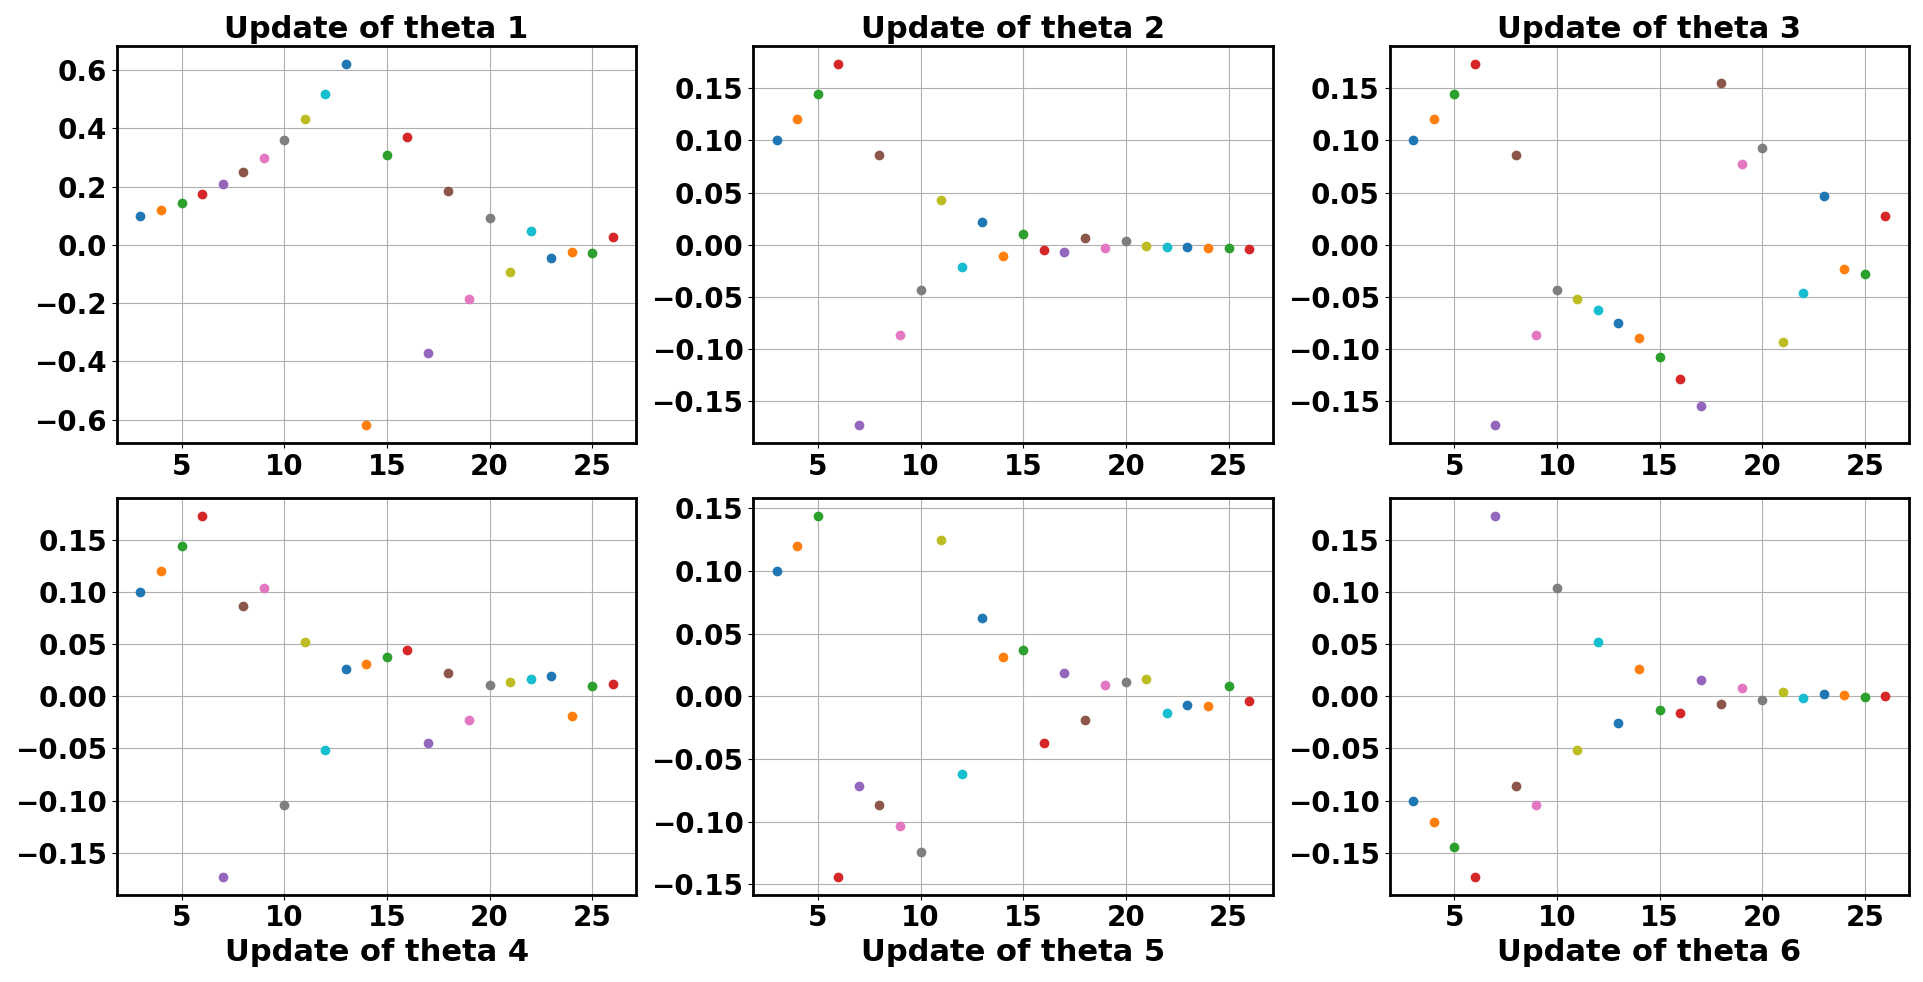
\includegraphics[width=1.0\textwidth]{15l.png}
	\caption{The difference of $\bm{\theta}$ with respect to one used in the previous iteration. }
	\label{fig:app_update}
\end{figure}


\begin{figure}[h!]
	\centering
	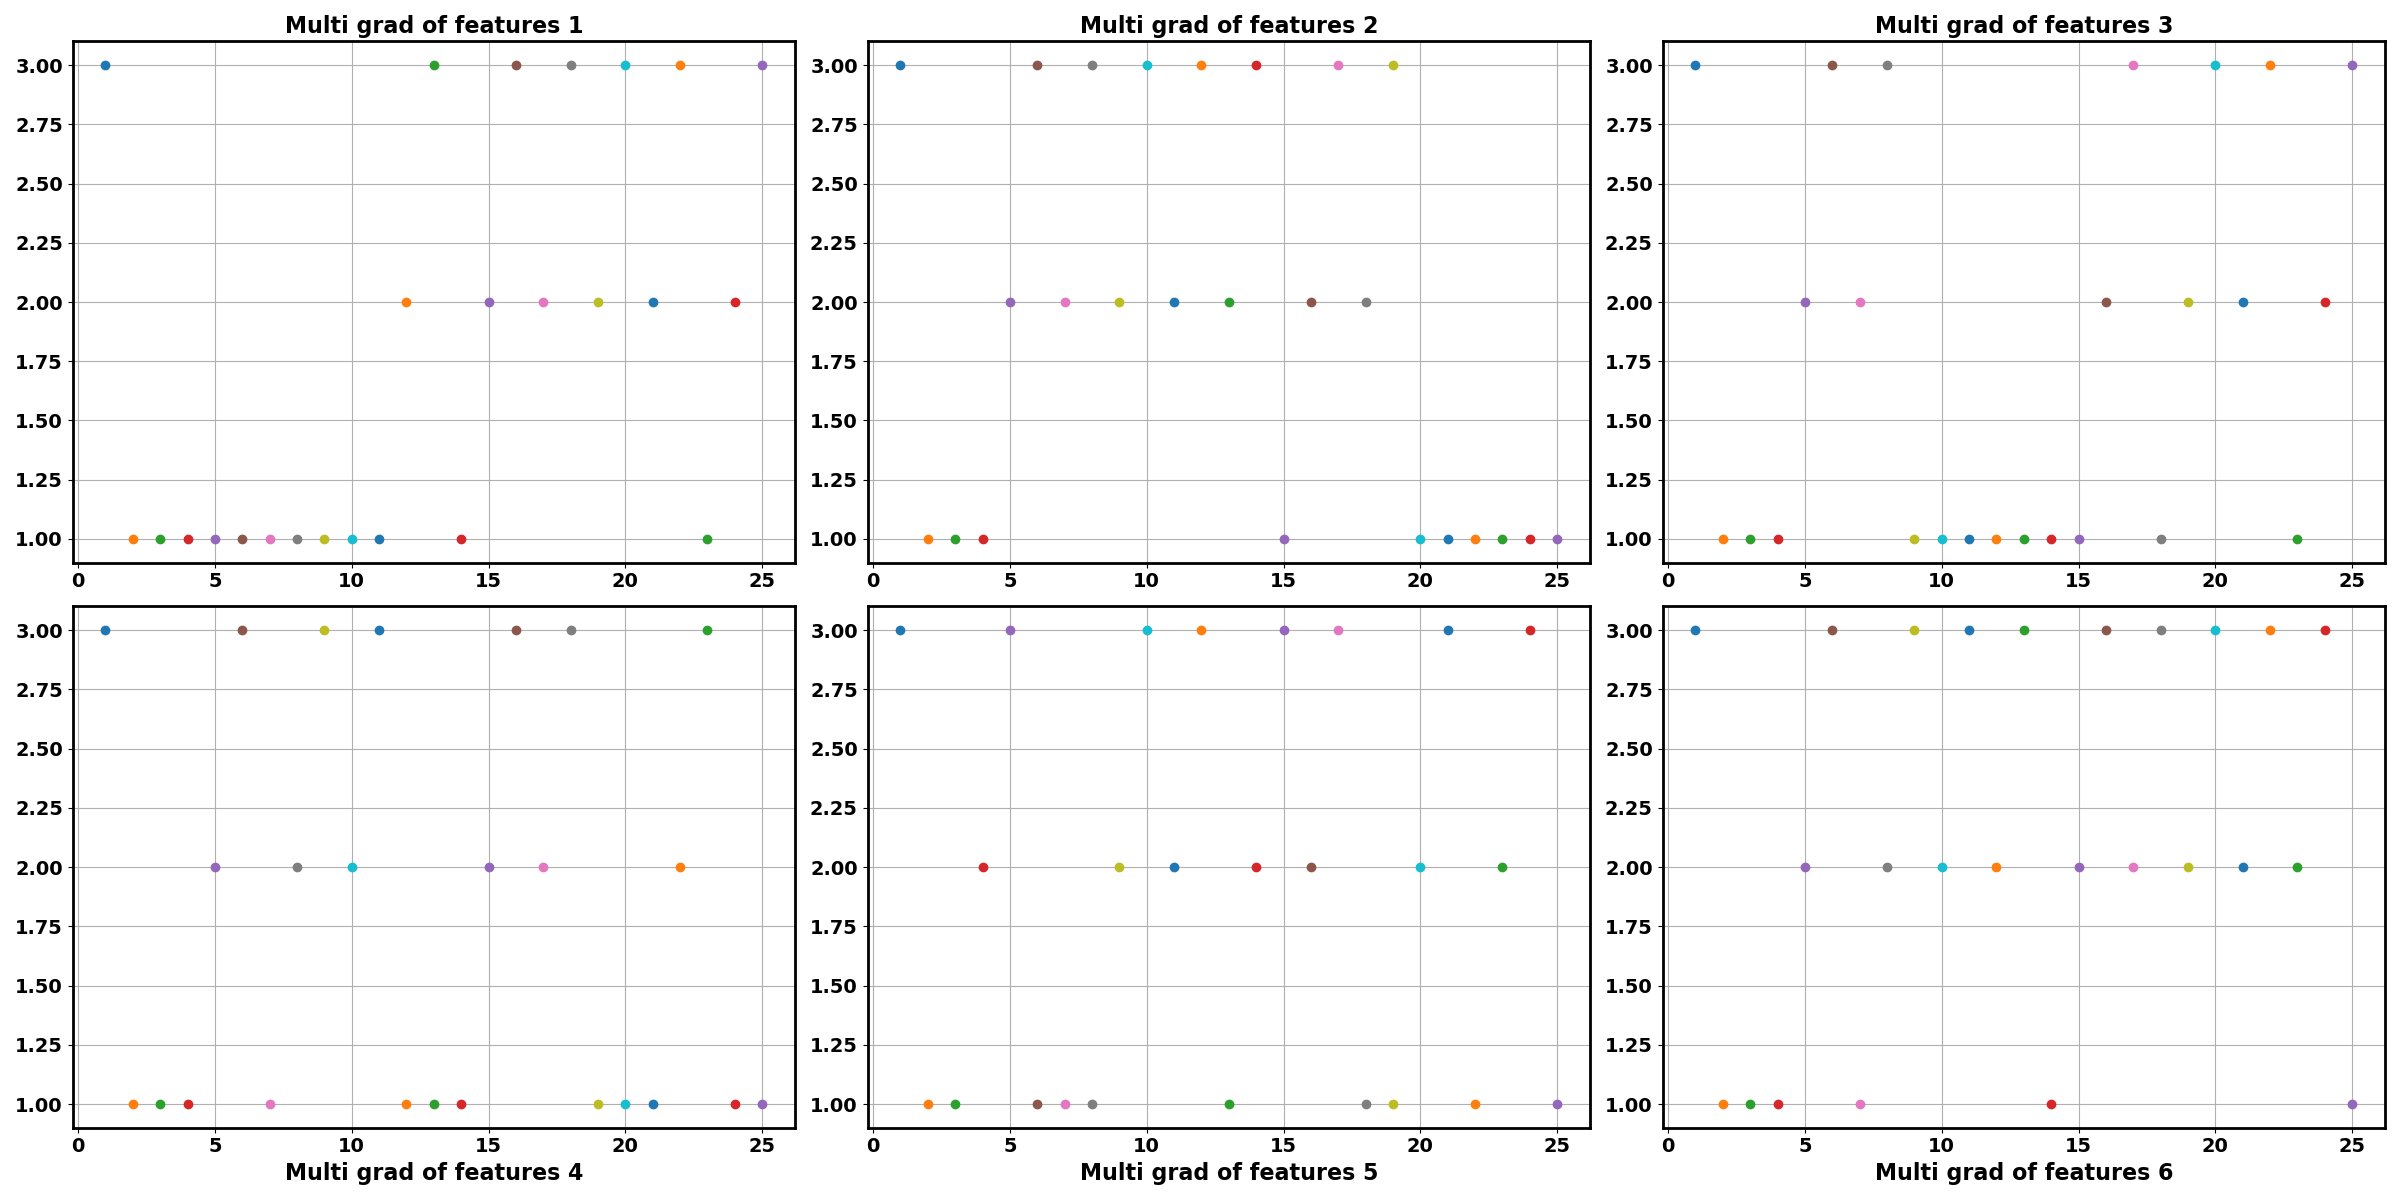
\includegraphics[width=1.0\textwidth]{16l.png}
	\caption{This figure shows which case of the three available in the RPROP algorithm is chosen during the learning iterations.}
	\label{fig:app_multigrad}
\end{figure}












%%% Local Variables: 
%%% mode: latex
%%% TeX-master: "thesis"
%%% End: 
